\chapter{Methodology}
\label{chap:methodology}

This chapter captures all methods that were used in the research to be able to answer the questions. It describes the collection of data through various sources, such as publicly available time series and field data that are recorded in this particular study. With these data are models made, which are used for answering the sub-questions which lead to the research question. 

\section{Data analysis existing data sets}
\label{sec:desk study}
In order to analyse and draw conclusions about the situation, the data sets used are explained in the following paragraphs. A summary is provided in Table \ref{tab:data collection summary}.

The first source of data is the National Institute of Water (INA). Since collaboration between TU Delft and INA is a central aim of this study, an “our data is your data” policy was applied, under which data are openly exchanged. Through this approach, INA provided a large number of datasets, which are presented in Table \ref{tab:data collection summary} to support the research. In addition, background knowledge about water discharge, erosion and negative impacts was shared in the form of publications and reports produced by INA staff and contacts. Furthermore, INA supplied geospatial datasets, including bathymetric surveys and a Digital Elevation Model (DEM) of the study area.

INA also directed us to a number of public sources for further hydrodynamic analysis and GIS applications. These included flow data from multiple gauging stations and publicly available bathymetric datasets. Examples are the Sistema Nacional de Información Hídrica (SNIH), point-based water level measurements from the governmental department Alerta, and water level records from the Prefectura Naval Argentina (PNA). An overview of these datasets is provided in Table \ref{tab:data collection summary}.
Finally, additional data were obtained through other stakeholder contacts. For example, the Dutch Embassy provided a case study on nature-based solutions (NBS) for the Paraguay River, while YPF supplied soil profile data related to dry sand mining activities in the Paraná region. More information on the approach with stakeholders can be found in Section \ref{sec:stakeholder methods}.

\begin{table}[H]
    \centering
    \renewcommand{\arraystretch}{1.2} % row spacing
    \setlength{\tabcolsep}{4pt}       % column padding
    \begin{tabularx}{\textwidth}{p{3.5cm}p{8cm}p{3.5cm}}
        \toprule
        Name & Description of data type & Source \\
        \midrule
        Comparative studies  & Background literature on geomorphology of similar areas & INA   \\
        INA Dataviewer         & Historical observations and simulations of water level and discharge time series & INA  \\
        DEM of lower Paraná & GeoTIFF file containing a Digital Elevation Model of the study area & INA \\
        Bathymetry (GIS) & Results from field campaigns in and around study area (2011, 2015, 2018) & INA \\
        Sand extraction permits & Agreements on locations and volumes of dredged sand & INA \\
        MarineTraffic & Live AIS vessel data & MarineTraffic \\
        Prefectura Naval Argentina  & Water level measurements & Prefectura Naval Argentina   \\
        Sistema Nacional de Informacíon Hídrica & Water level, discharge, fine and course sediment concentration & SNIH \\
        AquaMonitor & Deltares tool that represents water gains and losses based on historical satellite imagery & Deltares, Github, Google Earth Engine \\
        Bathymetry (pdf) & Detailed bathymetries along Paraná river in pdf-format & Secretaría de Transporte \\
        Google Earth & Tool that gives away satellite imagery of the globe. Can be used for a chosen time period of 1984-now & Google Earth  \\
        \bottomrule
    \end{tabularx}
    \caption{Summary of data sources}
    \label{tab:data collection summary}
\end{table}

\subsection{SNIH measurement stations}
\label{sec:measurementstations}
The measurement stations from the \textit{Sistema Nacional de Informacíon Hídrica} that were used for the data collection are discussed in this section. In order to have accurate estimations of the sediment content in the lower Paraná, it is interesting to consider its origin. As discussed in Section \ref{sec:origin sediment content}, most of the sediments in the middle Paraná originate from the Bermejo river in northern Argentina. A representative measurement station for this river is found near El Colorado, Formosa province. Here, the SNIH reports long series of measurements of water elevation, discharge and sediment concentrations.

Moving downstream, the Bermejo confluences with the Paraguay river. Merely 80 kilometers further downstream, the confluence of the Paraguay and Paraná river is located, near the city of Corrientes. Here, a drastic change in fluvial discharge occurs. Therefore, a station that represents the flow in the Middle Paraná is sought. Approximately 500 kilometers downstream of the confluence, the Túnel Subfluvial station near Santa Fe has a good amount of data. See Figure \ref{fig:rio parana map} for the location of El Colorado and Paraná (near Santa Fe). 

The two main tributaries of the Paraná that later flow into the Río de la Plata are the Paraná de las Palmas, and the Paraná-Guazú. To examine the distribution of discharge and sediment concentrations over these tributaries, two stations are selected and shown in Figure \ref{fig:flow partition}. First, the Zárate station is considered on the Paraná de las Palmas. On the Paraná-Guazú, the Brazo Largo station is selected for data analysis. Table \ref{tab:stations data collection} presents the data for all stations considered. Note that every dataset contains measurements of water level, discharge, fine sediment concentration and course sediment concentration. Most of the data is measured monthly, however some information is recorded on shorter time intervals. 


\begin{figure}
    \centering
    \includegraphics[width=0.75\linewidth]{figures/ch4/Flow partition1.png}
    \caption{Measurement stations of interest on Paraná de las Palmas and Paraná-Guazú}
    \label{fig:flow partition}
\end{figure}



\begin{table}[H]
    \centering
    \renewcommand{\arraystretch}{1.2} % extra row spacing
    \setlength{\tabcolsep}{8pt}       % extra column spacing
    \begin{tabular}{lllc}
        \toprule
        Station & SNIH ID & River & Data availability \\
        \midrule
        El Colorado         & 2602 & Bermejo               & 1968--2025 \\
        Túnel Subfluvial    & 3050 & Middle Paraná         & 1983--2025 \\
        Zárate              & 4001 & Paraná de las Palmas  & 1993--2025 \\
        Brazo Largo         & 4002 & Paraná-Guazú          & 1993--2025 \\
        \bottomrule
    \end{tabular}
    \caption{Selection of SNIH measurement stations.}
    \label{tab:stations data collection}
\end{table}



\subsection{Sand mining quantities}
The number of vessels involved in river dredging activities on the Paraná Guazú was determined using AIS (Automatic Identification System) data. Vessel movements between dredging sites and ports were monitored through \textit{MarineTraffic}. Although historical records were not considered, the daily activity observed during the study period provides a reliable estimate of the sand extraction volumes. 

Alternatively, a collection of dredging permits in the river is considered. To avoid adverse impacts on the hydraulic regime of the river due to dredging, companies must first obtain permits from the \textit{National Water Institute }(INA). These permits specify the locations and volumes of the proposed dredging activities. The information they provide serves as a reliable estimate of the total material being removed from the river, thereby influencing the sediment balance. Therefore, the permits were analysed for the area of interest.
Subsequently, the information gathered from AIS data and extraction permits were combined, resulting in estimates of volumes that are dredged in the study area. In addition, conversations with stakeholders were of valuable insight and supported the comparison with the results of the data collection.

The information about dry sand mining is however gained through different sources. The main sources were a literature review and the semi-structured interviews (which are explained Section \ref{sec:stakeholder methods}. These were used to gather data on dry sand mining quantities, usage purposes, and the factors influencing demand for sand from the region. The literature review provided background and quantitative information, while interviews offered insights from stakeholders directly involved in sand extraction and use.

\section{Field study}
\label{sec:field study}
The goal of the field work was to obtain data from measurements on the boat using different devices, as well as obtaining resourceful information from chosen stakeholders in the area of the field work. This data would then be filtered, analysed and used to take give answers on the research question of the report.

The field work divided the group of six students in two, leaving one group of three on the boat with two supervisors of INA to take the required measurements, and one group of three with another colleague of INA for the interviews.

\subsection{Stakeholders}
\label{sec:stakeholder methods}
In this study qualitative research was conducted to explore perceptions and experiences related to the river. For this, interviews were conducted to capture insights from participants with diverse perspectives.

A qualitative approach was chosen because it allows for a detailed understanding of participant's views and interpretations of the river. This design is particularly suited to capture the complexity of social and environmental issues and to highlight the ways in which different stakeholders experience and assign meaning to the river.Data were collected through semi-structured interviews, a method that combines prepared guiding questions with the flexibility to follow up on unexpected but relevant topics raised by participants. This format ensured that key themes were consistently addressed in interviews while also allowing interviewees to elaborate on issues they considered important. In practice, a topic guide with questions per stakeholder was developed to provide structure, but the interviewer encouraged open-ended responses and probed further where clarification or depth was needed. During the interview, responses were written down in key words. The prepared questions for the specific stakeholders are given in Appendix \ref{chap:interviews}.

In case of language barriers the questions and responses are translated. Most stakeholders were approached by mail to get in contact and reached on-site. After each interview, permission is asked to quote and name the stakeholder in the report. Table \ref{tab:stakeholders} gives an overview of the stakeholders who were contacted, when and by what method. 

\begin{table}[H]
    \centering
    \begin{tabularx}{\textwidth}{l l l}
        \toprule
        Date & Occupation & Method \\
        \midrule
        12-09-2025 & Fishers & Mail \\
        12-09-2025 & Ports & Mail \\
        12-09-2025 & Filmmakers & Whatsapp \\
        24-09-2025 & Landowners & Whatsapp and On-site \\
        25-09-2025 & Agencia Nacional de Puertos y Navegación (ANPYN) &  Mail \\
        25-09-2025 & Dredgers & On-site \\
        25-09-2025 & Camping owner & Mail and On-site \\
        30-09-2025 & Prefectura Naval Argentina (PNA) & Mail \\
        \bottomrule
    \end{tabularx}
    \caption{Stakeholder overview}
    \label{tab:stakeholders}
\end{table}

% TABEL AANPASSEN. WIE HOE WANNER. LOCATION AND LANGUAGE NAAR DE RESULTATEN. OOK DE BENAMING SPECIFIEK IN DE RESULTATEN BENOEMEN EN HIER ALGEMEEN BLIJVEN. EXTRA KOLOM HOE TEOVOEGEN; MAIL, WHATSAPP, TEAMS

\subsection{Measurement variables and equipment}
\label{Measurement variables and equipment}
In this section are the location and type of measurements explained. The goal of the field work was to obtain data from critical sections in the study area. These locations were selected in such a way that they were as useful as possible for establishing the sediment balance. Two important locations in the study area are the confluence from the Ibicuy and Paraná Guazú, and that of the Paraná Guazú and Talabera. In these sections, sediment samples and flow measurements were recorded.
Once this data was gathered, it was analysed and compared to previously obtained data to draw conclusions. 


% \begin{figure}[H]
%     \centering
%     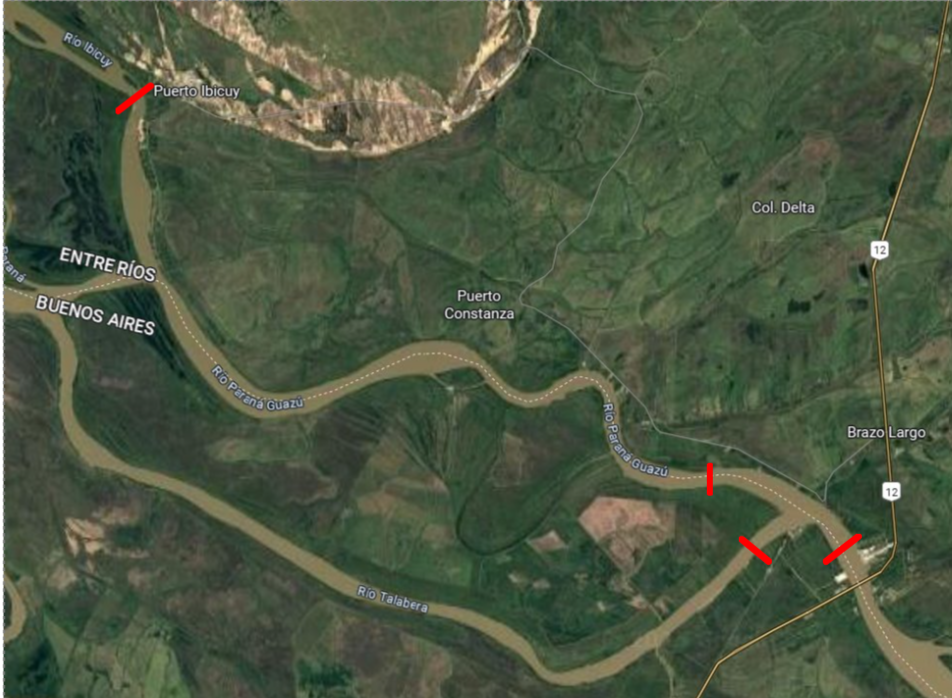
\includegraphics[width=0.5\linewidth]{figures/ch4/Critical measurement points.png}
%     \caption{Critical Cross Section Measurements}
%     \label{fig:fieldwork cross sections}
% \end{figure}

% The program of the boat days consisted of going over the indicated critical cross sections (in red on Figure 4.2) a total of 4 times, using the equipment of INA to save the necessary information of the river. 


Firstly is the Flow velocity measured profile of the river. This is recorded by a SonTek RiverSurveyor M9 Acoustic Doppler Current Profiler (ACDP). This device consists of two components both placed on a floating board held next to the boat while advancing. The components are a vertical acoustic echo sounder beam placed on the back end of the floating board, and a rectangle shape box containing a microprocessor that computes the data on the front end of the board, as seen in Figure \ref{fig:SonTekmeasurement}.

\begin{figure}[H]
    \centering
    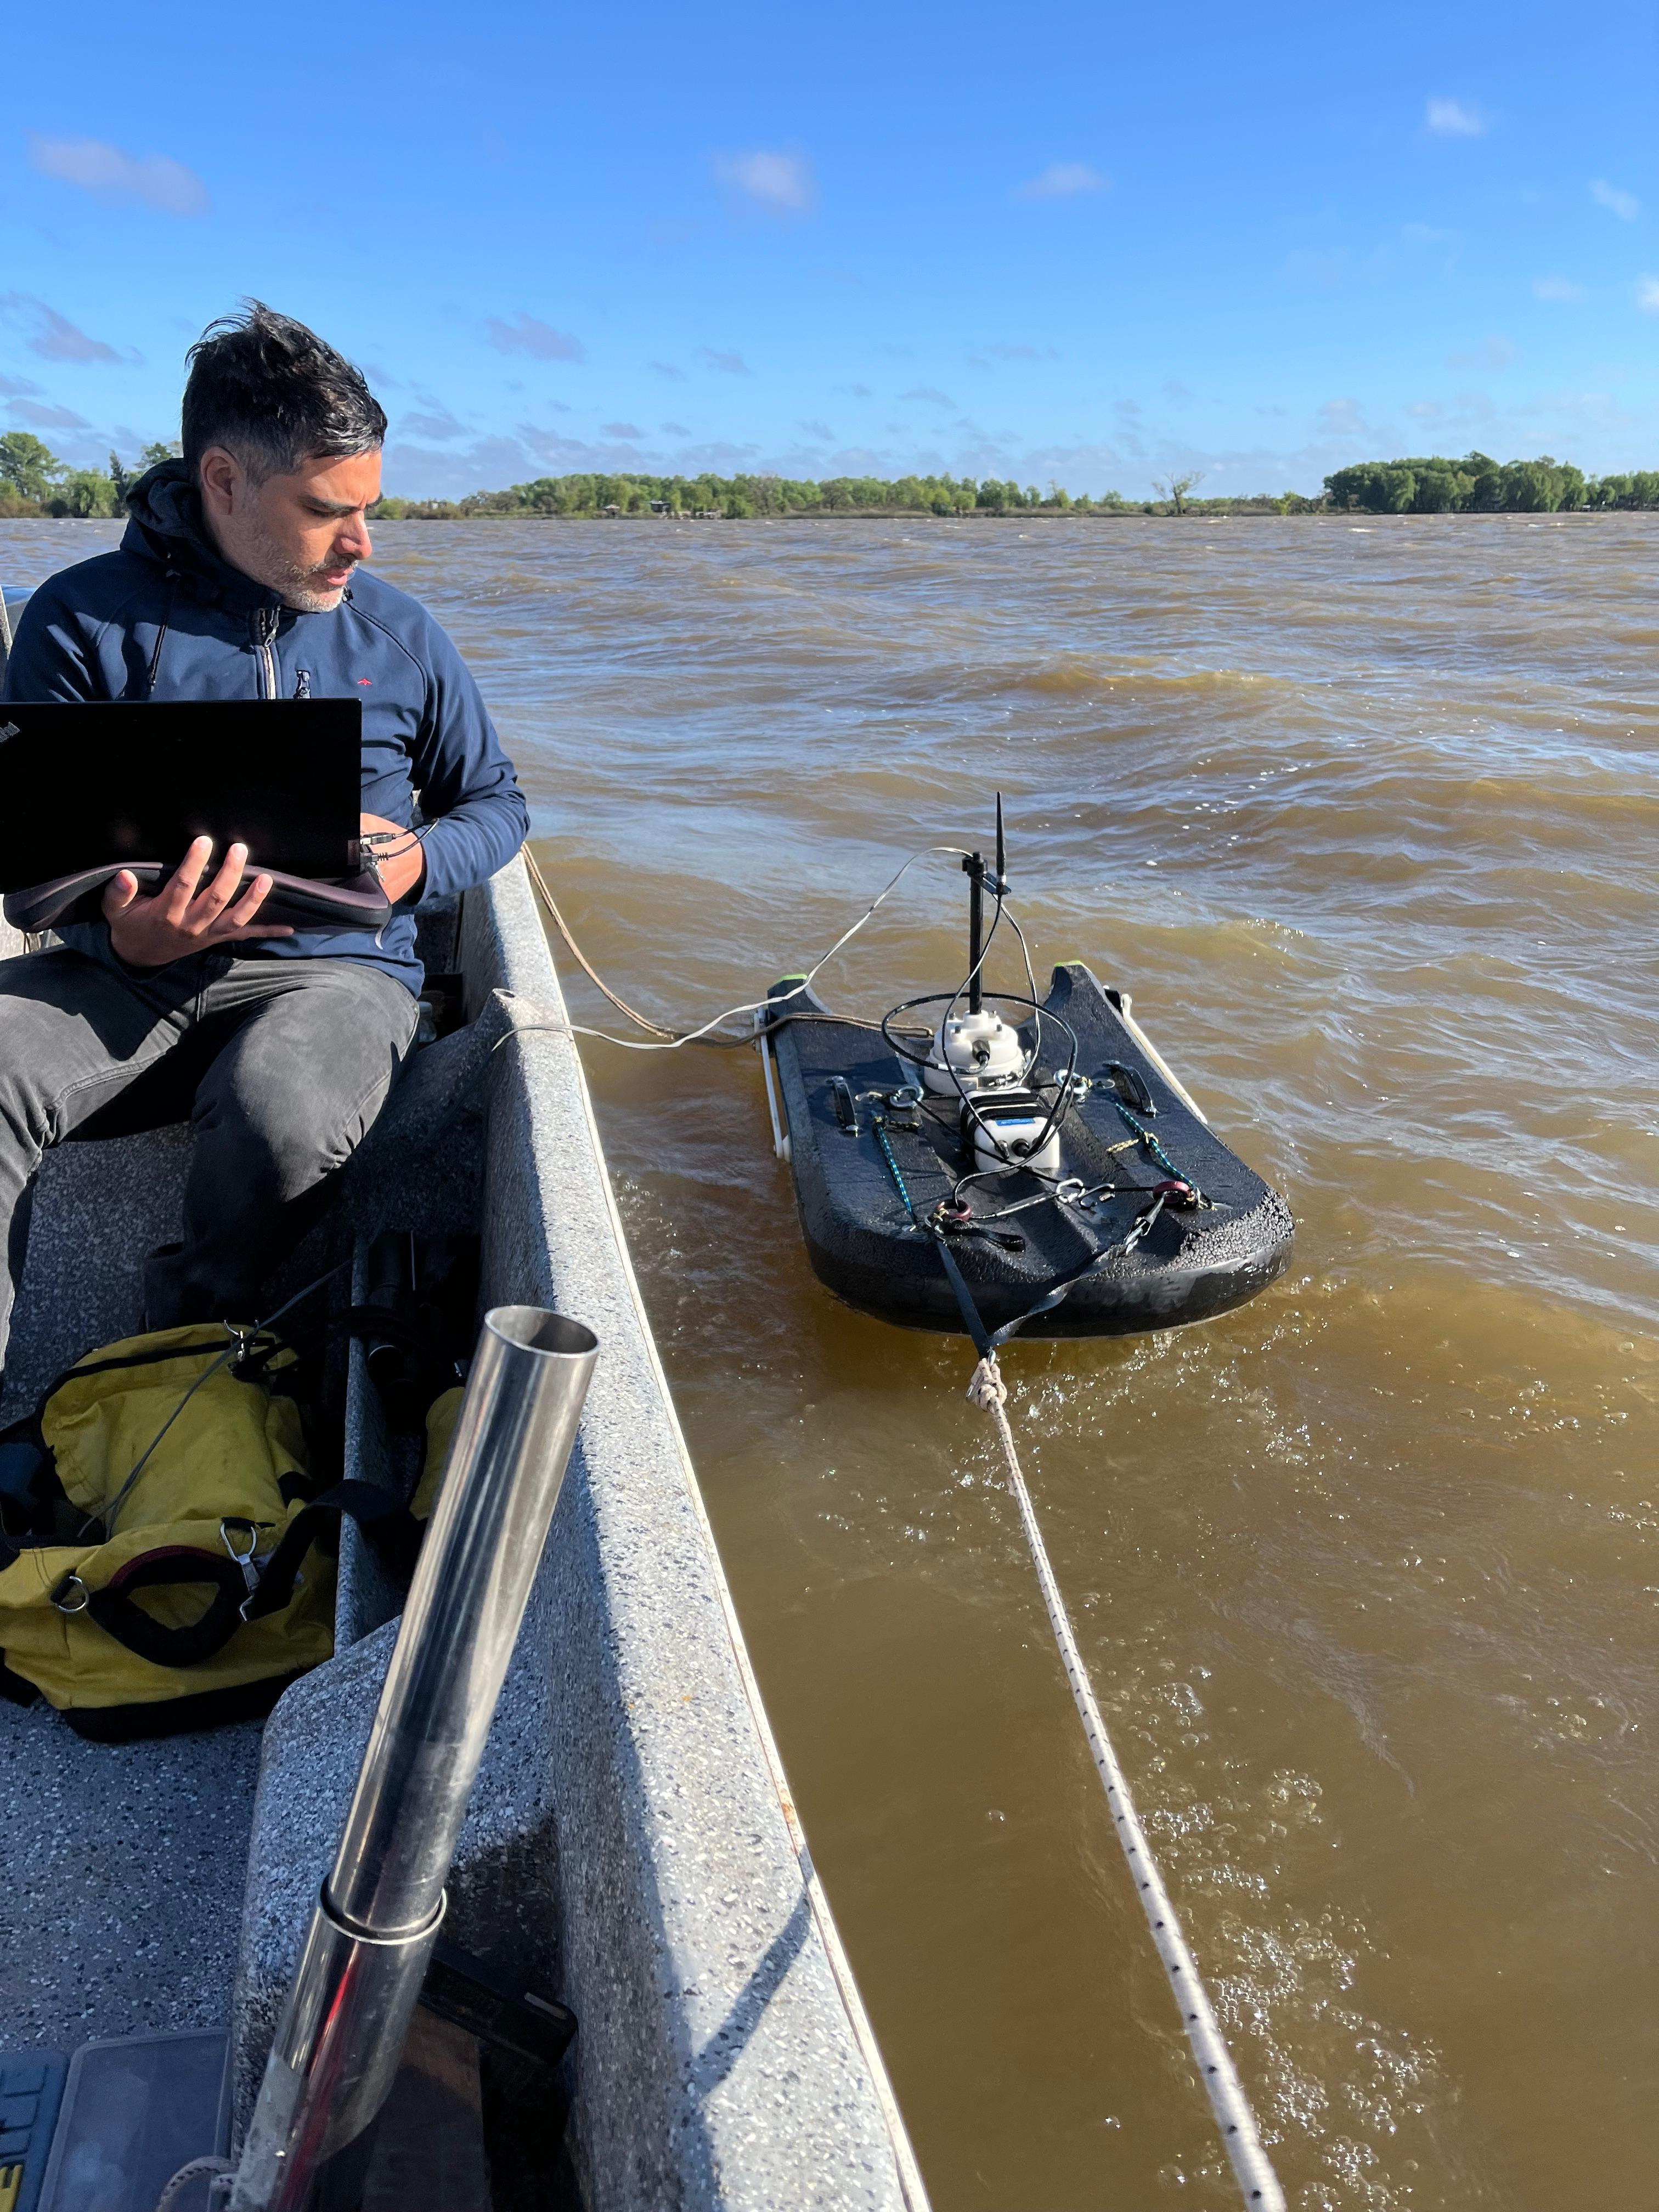
\includegraphics[width=0.5\linewidth]{figures/ch4/sonteknico.jpg}
    \caption{SonTek M9 installed in the field}
    \label{fig:SonTekmeasurement}
\end{figure}

The speciality of the SonTek M9 is that it uses multiple acoustic frequencies to find a high resolution range of depths and flow velocities, while still tracking the geo-referenced position of the vessel using GNSS \autocite{ysiinc.SonTekM9}. The flow velocity is the speed of the river in a certain direction. The unit is therefore  [m/s], and is expressed in the form of a vector. The significance of this data is also due to the fact that the velocity is needed to compute the discharge as well.

Secondly the bathymetry is found using two different methods. The ADCP and the Garmin echosounder were used for this. The bathymetry is the depth of the channel at the position of the boat on a given timestep. Moving over the whole width of the channel yields a longitudinal profile, indicating what depth lies at what coordinates.
The echosounder is attached to a pole on the side of the boat, and dipped into the water while the boat is moving. This pole is connected to the Garmin screen giving the depth and bathymetry of the channel, as seen in the Figure \ref{fig:Garmin}. In addition, this screen allows monitoring of possible bed forms in the river bed. The profile was taken on the whole trajectory between Puerto Guazu to Ibicuy in the morning upstream, and downstream on the end of the afternoon. This profile is seen in Figure \ref{fig:measurements day2}.

\begin{figure}[H]
    \centering
    \begin{subfigure}[b]{0.48\textwidth}
        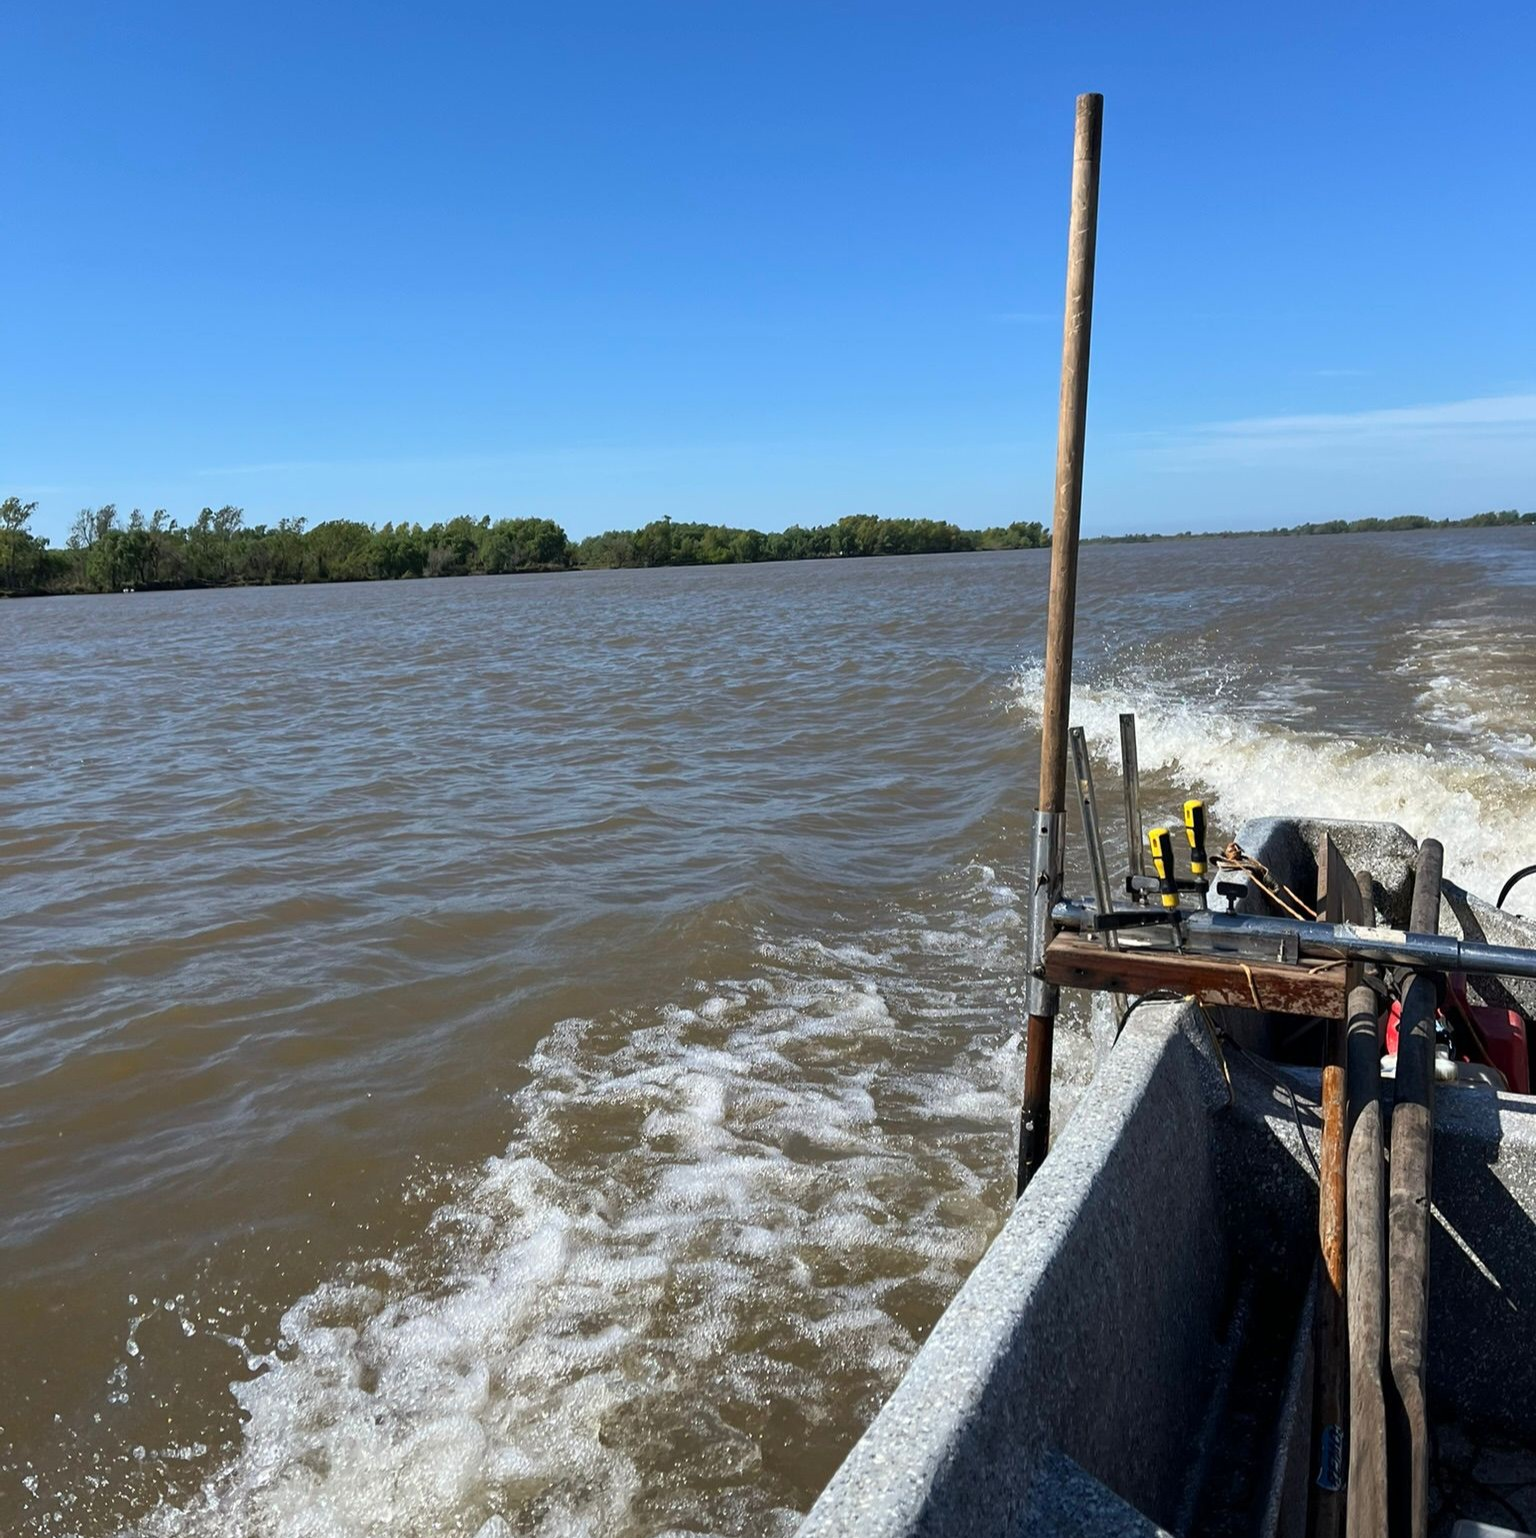
\includegraphics[width=\linewidth]{figures/ch4/Echosounder.jpg}
        \caption{Echosounder attached to boat}
        
    \end{subfigure}
    \hfill
    \begin{subfigure}[b]{0.48\textwidth}
        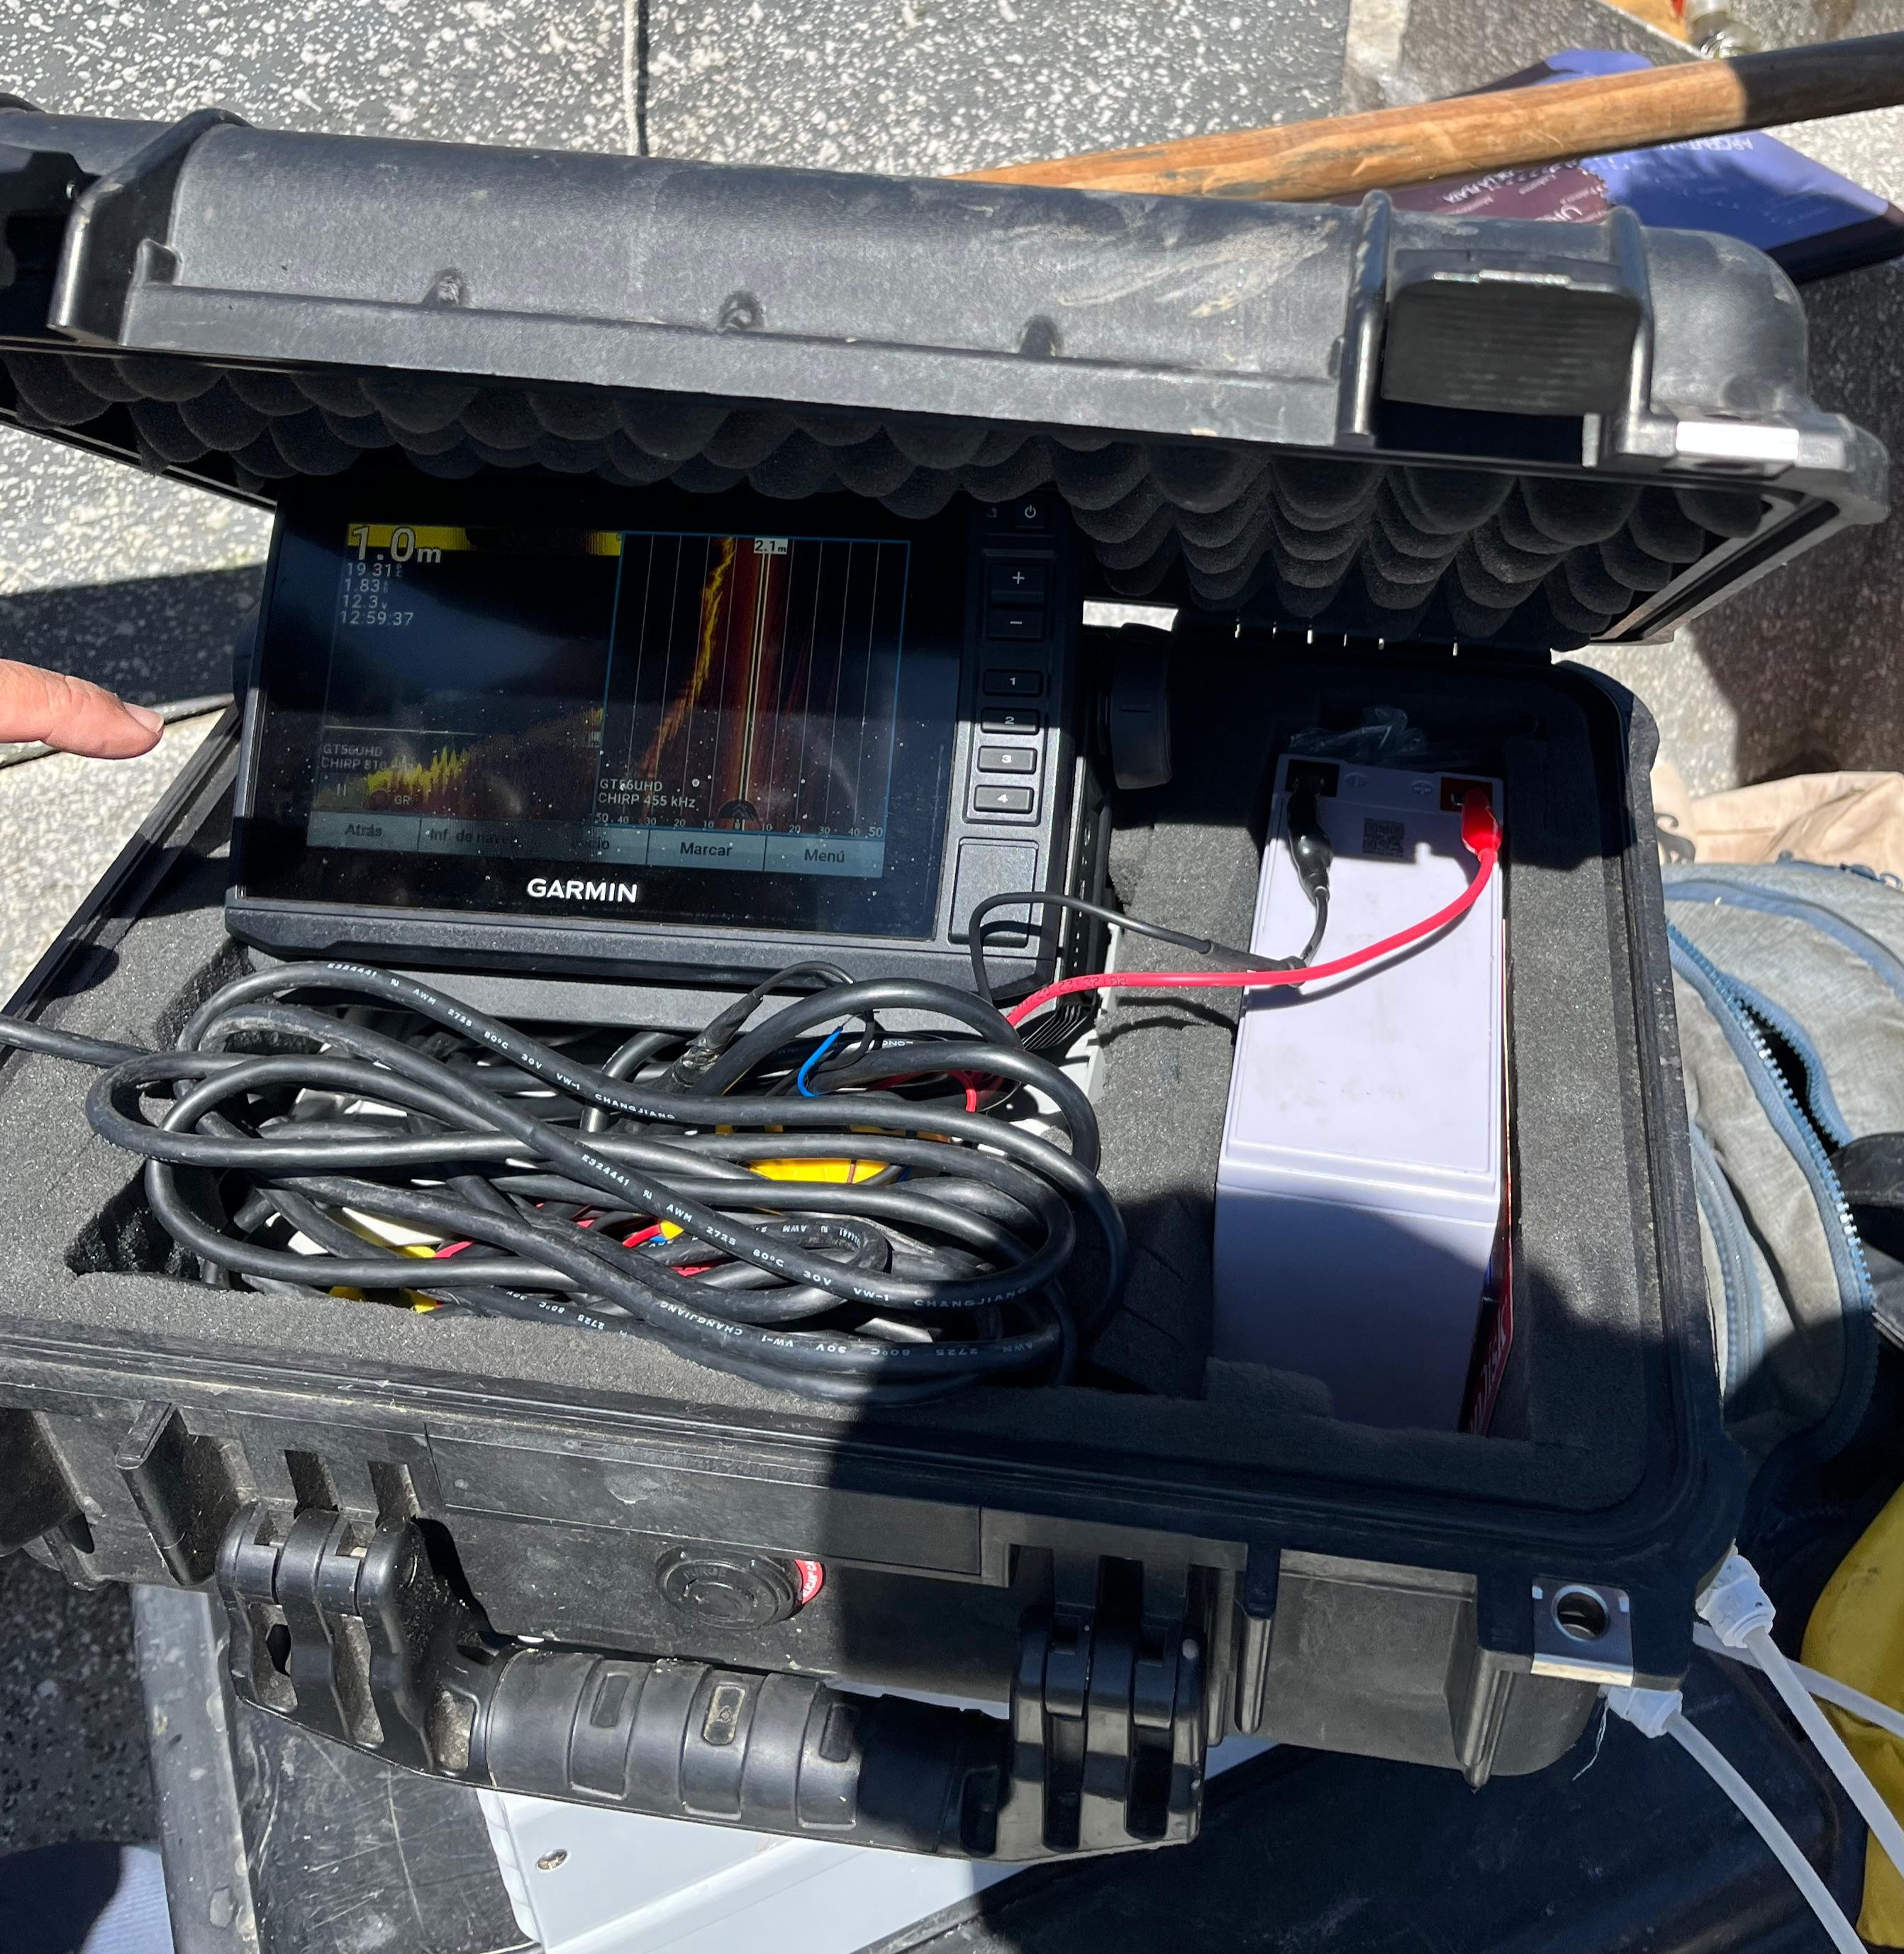
\includegraphics[width=\linewidth]{figures/ch4/garmin.jpg}
        \caption{Garmin material}
        
    \end{subfigure}
    \caption{Echosounder and Garmin measurements}
    \label{fig:Garmin}
\end{figure}


From the Bathymetry and the flow velocity is the Discharge researched. The flow velocity \(\mathbf{v}\) is integrated over the depth and the width of the channel (through a cross-section) which in the end yields the discharge \(Q\) of the river at a given location, with a unit of \si{\cubic\metre}/s.
\begin{equation}
    Q = \iint_A \mathbf{v} \cdot d\mathbf{A}
    \label{eq:discharge_integration}
\end{equation}

\noindent where:
\begin{itemize}
    \item \(Q\) is the discharge, expressed in cubic meters per second [m\textsuperscript{3}/s];
    \item \(\mathbf{v}\) is the flow velocity vector, expressed in meters per second [m/s];
    \item \(A\) is the cross-sectional area perpendicular to the flow, expressed in square meters [m\textsuperscript{2}];
    \item \(d\mathbf{A}\) is an infinitesimal area element.
\end{itemize}

The number of required measurements of a single cross section is defined by the variability of the measurements. That is, a minimum of two measurements exists, which is sufficient when the second discharge measurement is within 10\% of the first one. In addition, correct operation of the vessel's velocity is essential for reliable discharge results. Therefore, the boat speed should never exceed the flow velocity perpendicular to the cross section under consideration. 



% The aim of the field work was to obtain the data of flow velocity and discharge at the three critical points around the bifurcation of interest during different times, one in the morning and in the afternoon. Consequently this would indicate some changes in discharge for different times, flows, circumstances hence solidifying our data base of examples. 



Thirdly, it is in the report's interest to gather data on the suspended sediment concentration of the river. This is done by collecting water with the help of an APEMA BS6A peristaltic pump connected to two plastic tubes. The first tube is short and is used to insert the water into the plastic bottles on the boat. The second tube is long and is connected to a weight, which can be lowered into the river to a certain depth. At the desired depth, the fluid was pumped to the water surface and collected in the plastic bottles.

Then, the samples were sealed in order to be sent to the water quality lab in the hydraulic section on the INA site, as seen in Figure \ref{fig:suspended-sediment}. These samples help to indicate the concentration of fine sediments in the channel, at different locations and elevations. The evolution of the concentrations along the study area will be studied in Chapter \ref{chap:hydroanalysis}.

\begin{figure}[H]
    \centering
    % Left image
    \begin{subfigure}[t]{0.48\textwidth}
        \centering
        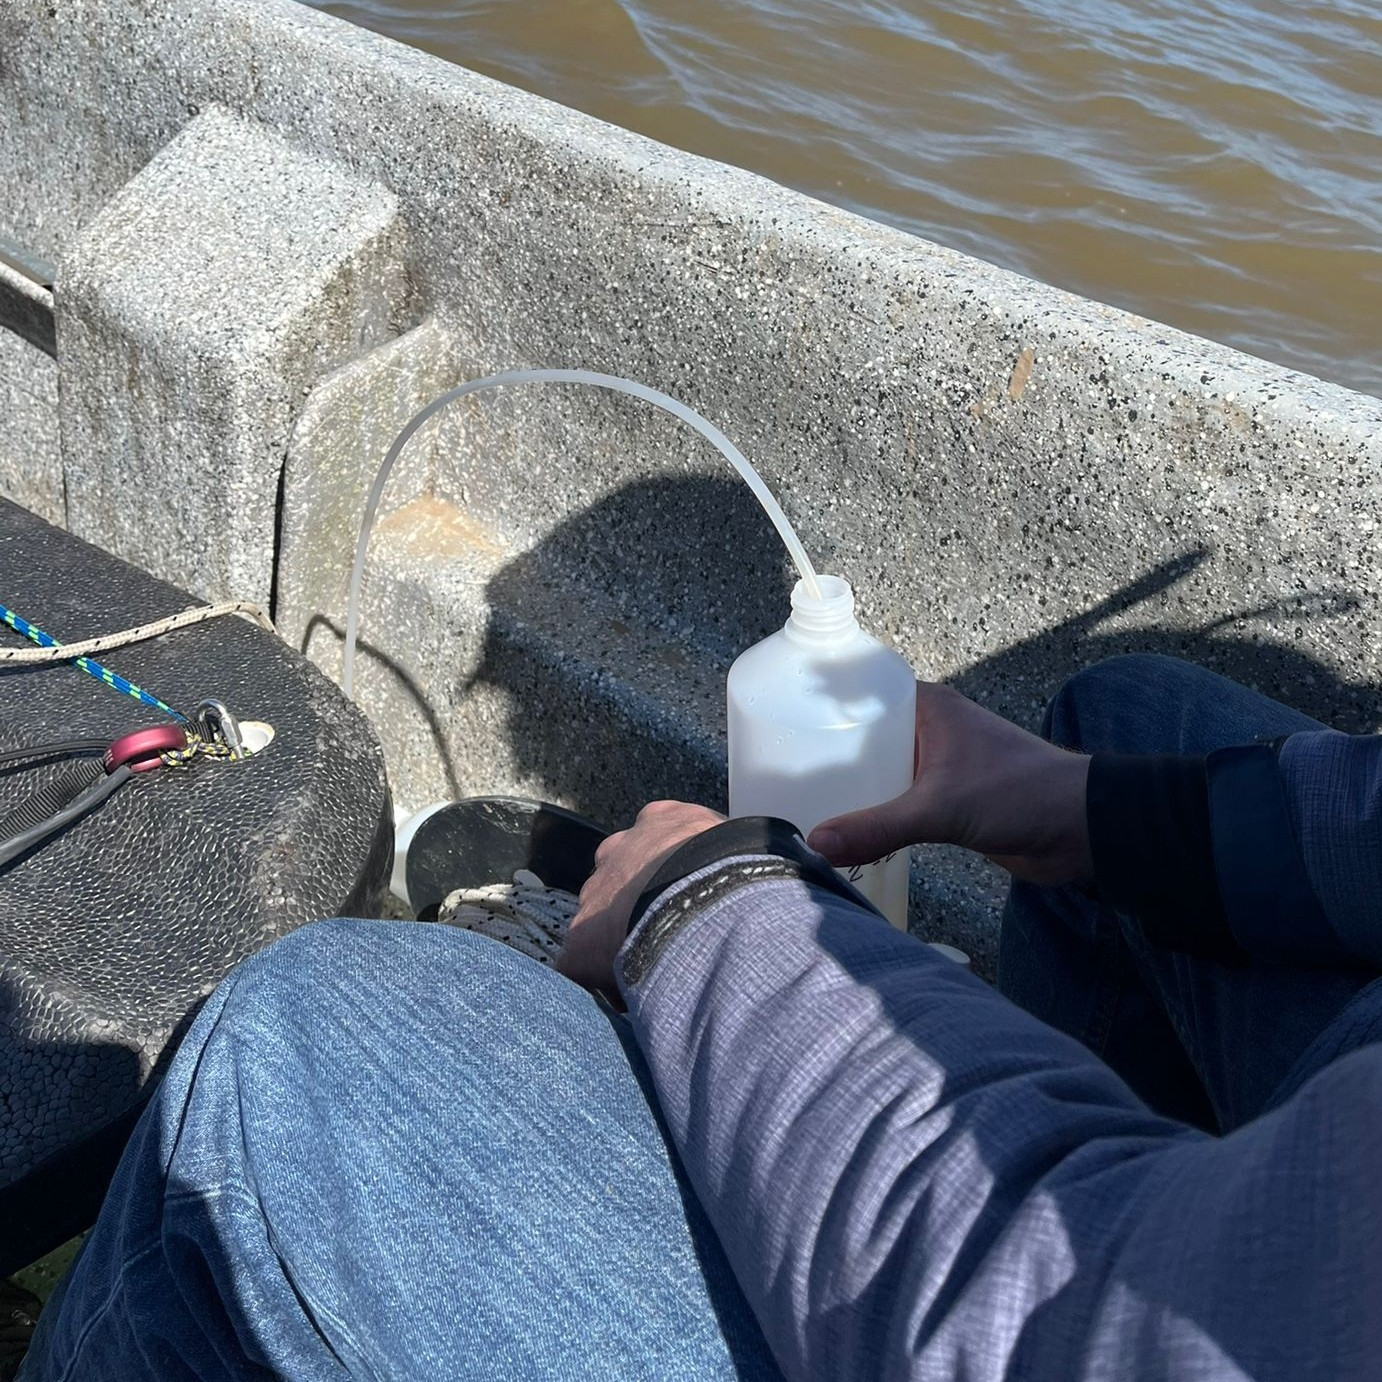
\includegraphics[width=\linewidth]{figures/ch4/fles.jpg}
        \caption{Filling the samples}
    \end{subfigure}
    \hfill
    % Right image
    \begin{subfigure}[t]{0.48\textwidth}
        \centering
        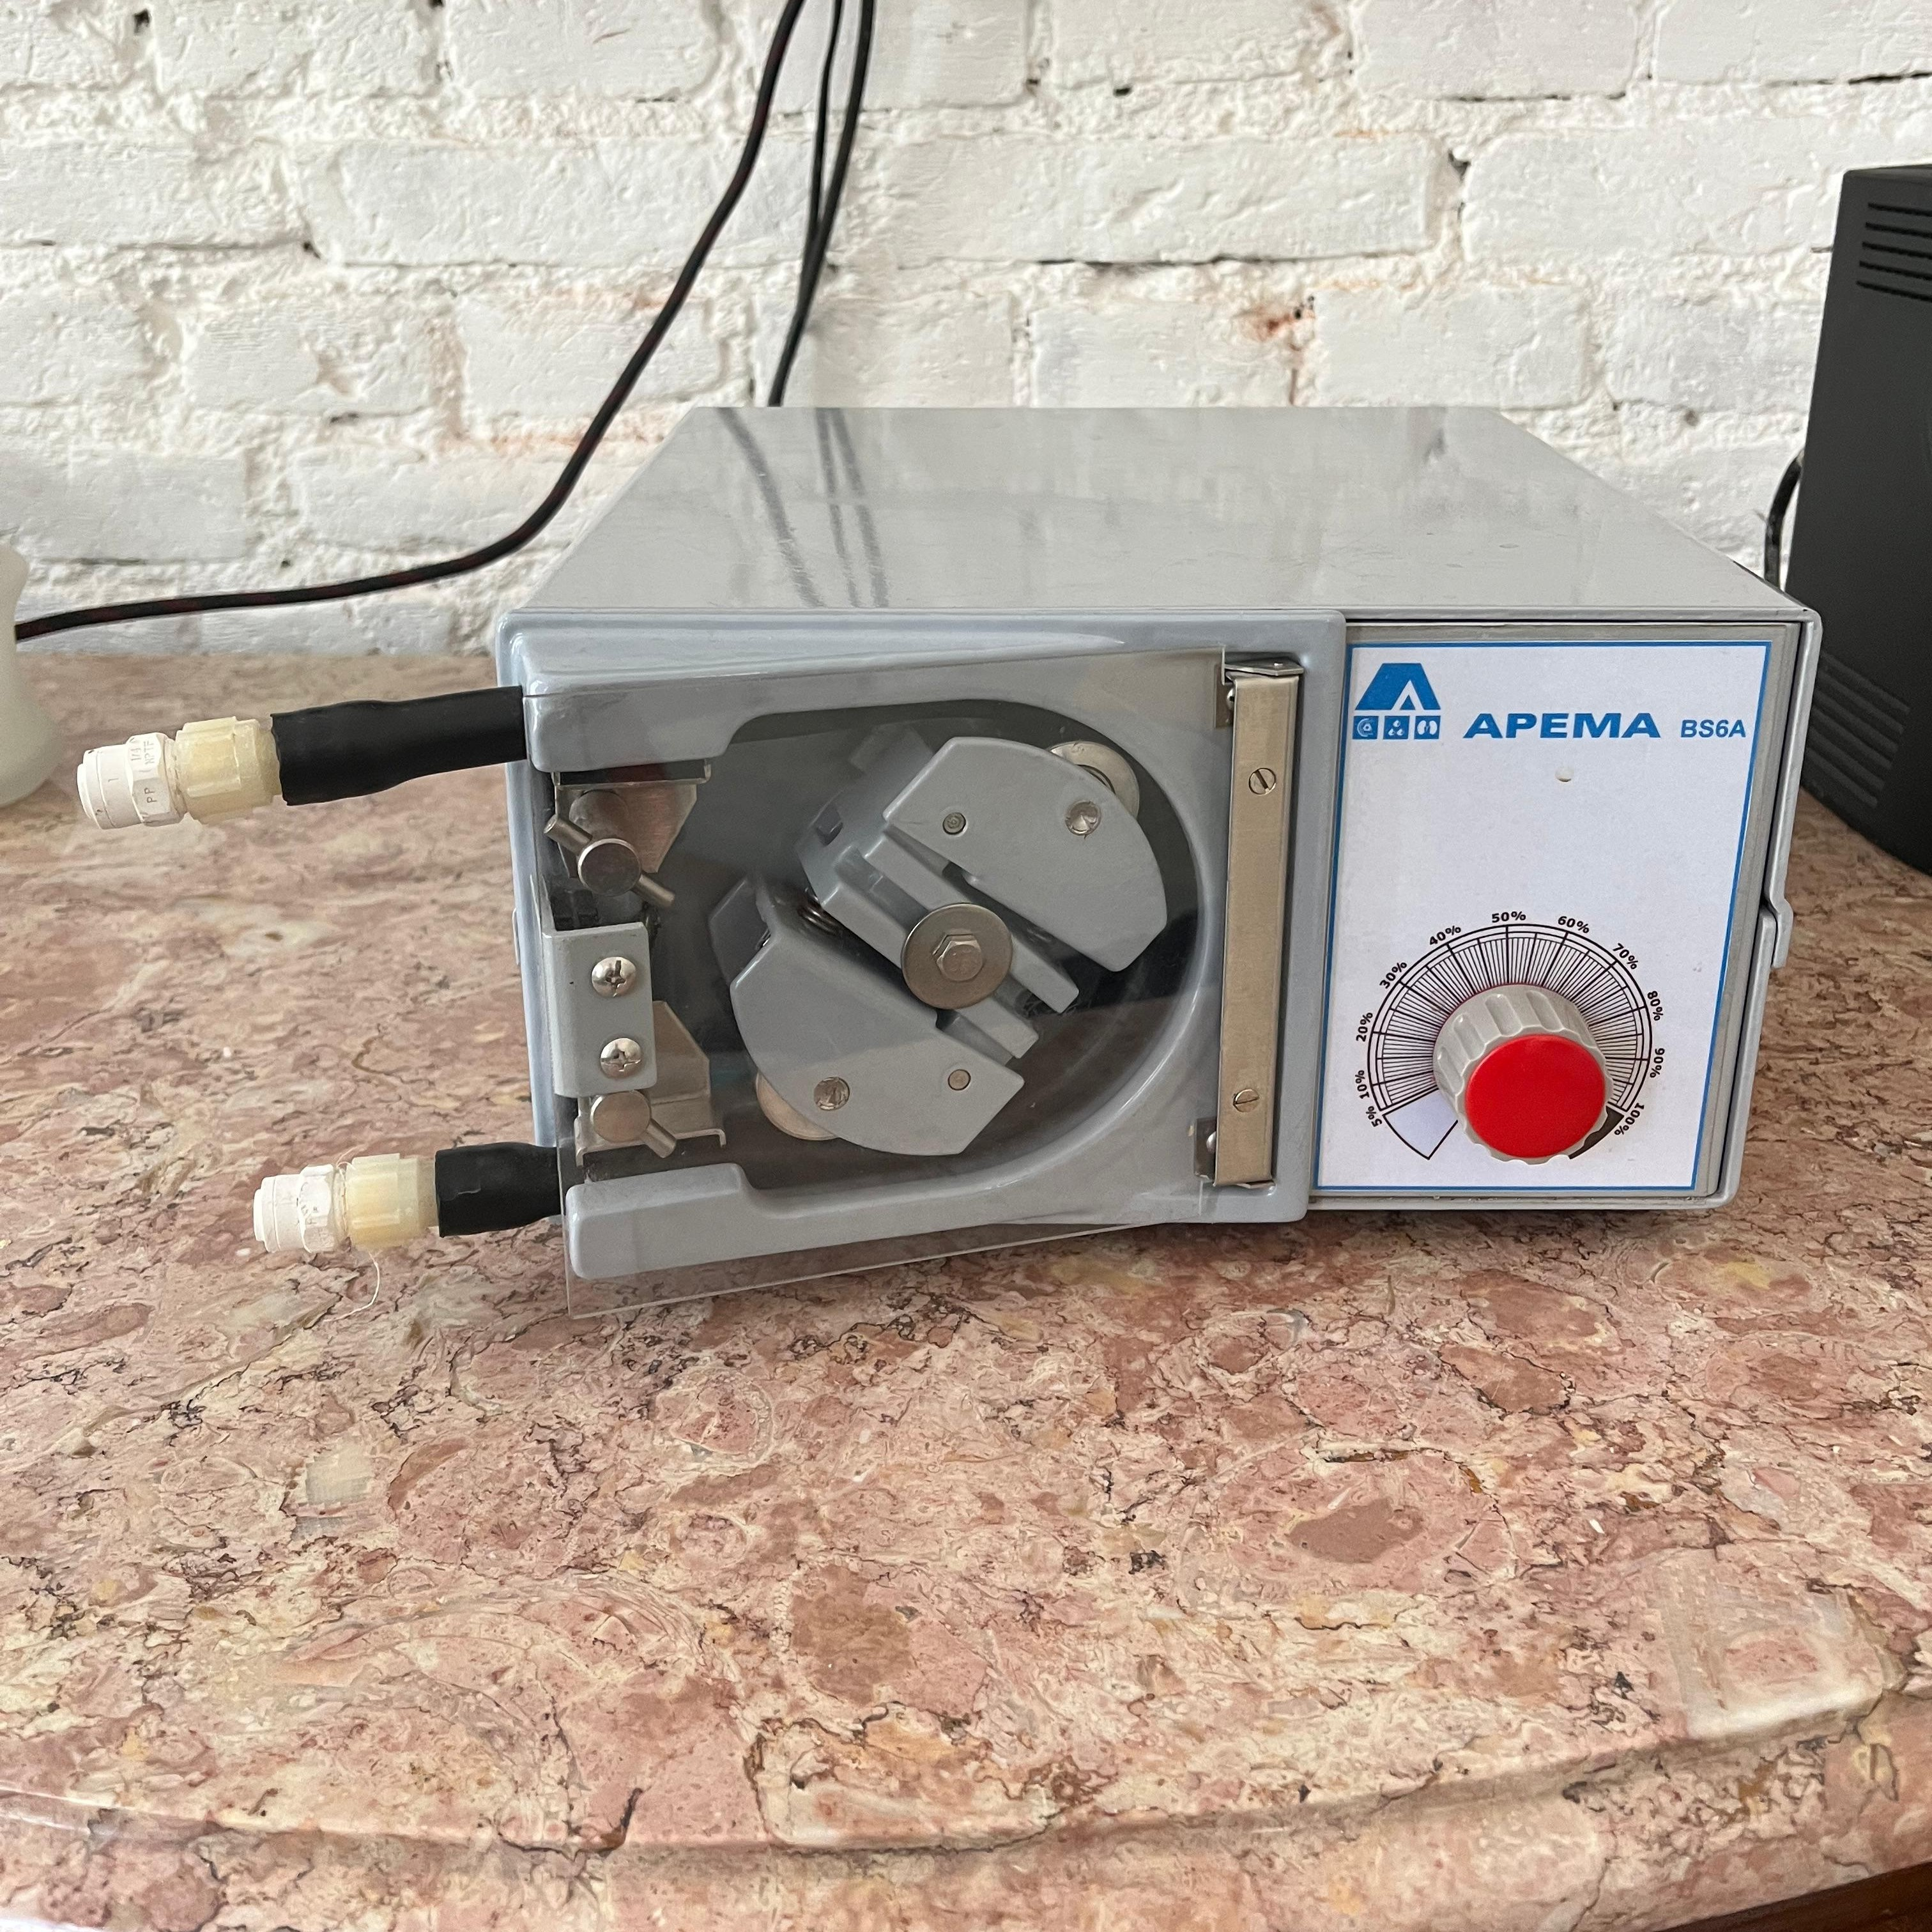
\includegraphics[width=\linewidth]{figures/ch4/APEMA BS6A.jpg}
        \caption{APEMA BS6A device}
    \end{subfigure}
    \caption{Suspended sediment measurements}
    \label{fig:suspended-sediment}
\end{figure}




% In theory, since it was done at different levels of the river, it could potentially indicate a change in concentration from one point upper at Ibicuy to Brazo Largo in the southern, lower part of the study area. From this data, the group could draw even further conclusions.


Fourthly, the bed load was a necessary measurement for the complete analysis. The method used for this parameter is scraping the bottom layer of the channel with a metal shaped container. The goal is to retrieve samples that represent the granulometry of the bed at different depths. 
The strategy for this measurement is tying a rope to the metal container, dropping it until it reaches the maximum depth of the location. Then, with help of the current or the boat, the person who holds the rope drags the container along with the horizontal movement which gradually collects sediment from the surface. Once this is done, the rope and the container are pulled up and restored in the boat. The last step is to collect some sediment and put it in a plastic bag.  Later on, the captured sediment was sent to the lab where the soil was dried out to find the components, quality and other parameters of the soil such as porosity which would add up to the results. The metal container, as well as the extracts of the sediment samples in the oven are shown in Figure \ref{fig:bed-load}. 

\begin{figure}[H]
    \centering

    % First (large) image
    \begin{subfigure}{0.7\textwidth}
        \centering
        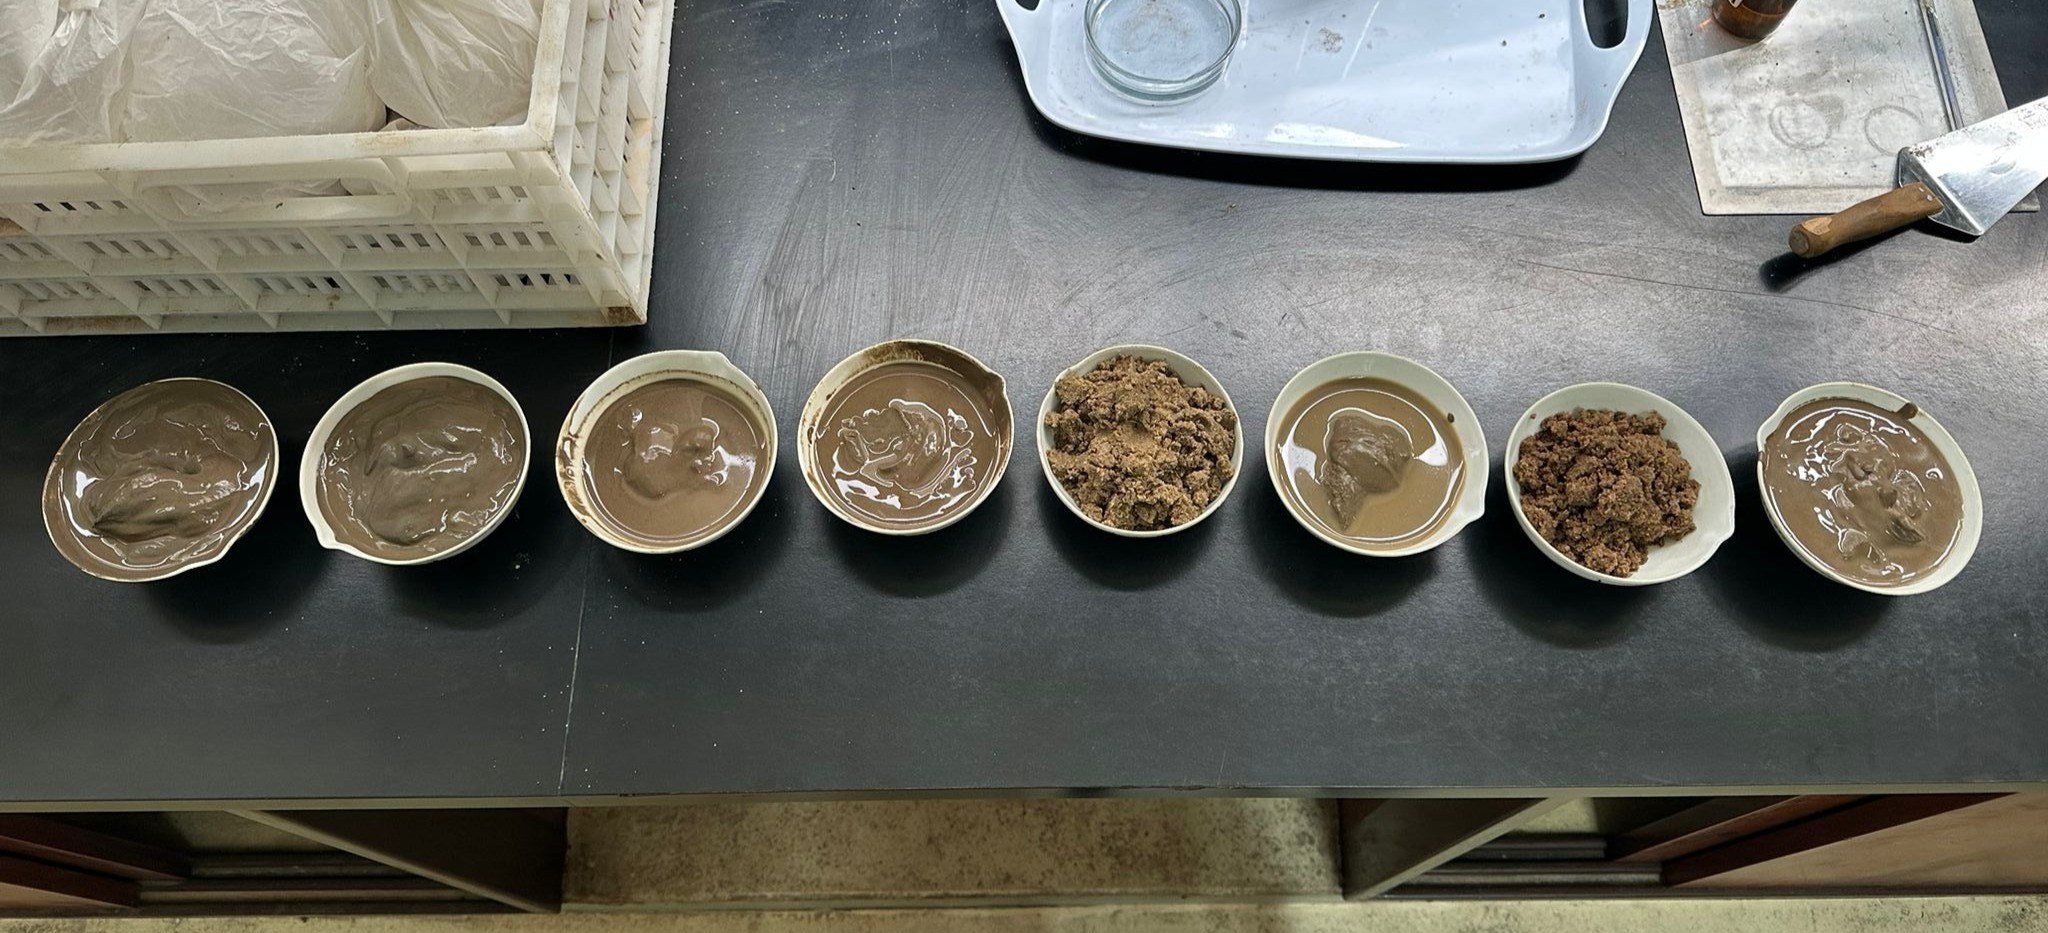
\includegraphics[width=\linewidth]{figures/appendixE/soilsamples.jpg}
        \caption{Bed Load Samples from the Fieldwork}
    \end{subfigure}

    \par\vspace{0.5cm} % use this instead of \vspace alone

    % Two smaller images side by side
    \begin{subfigure}{0.48\textwidth}
        \centering
        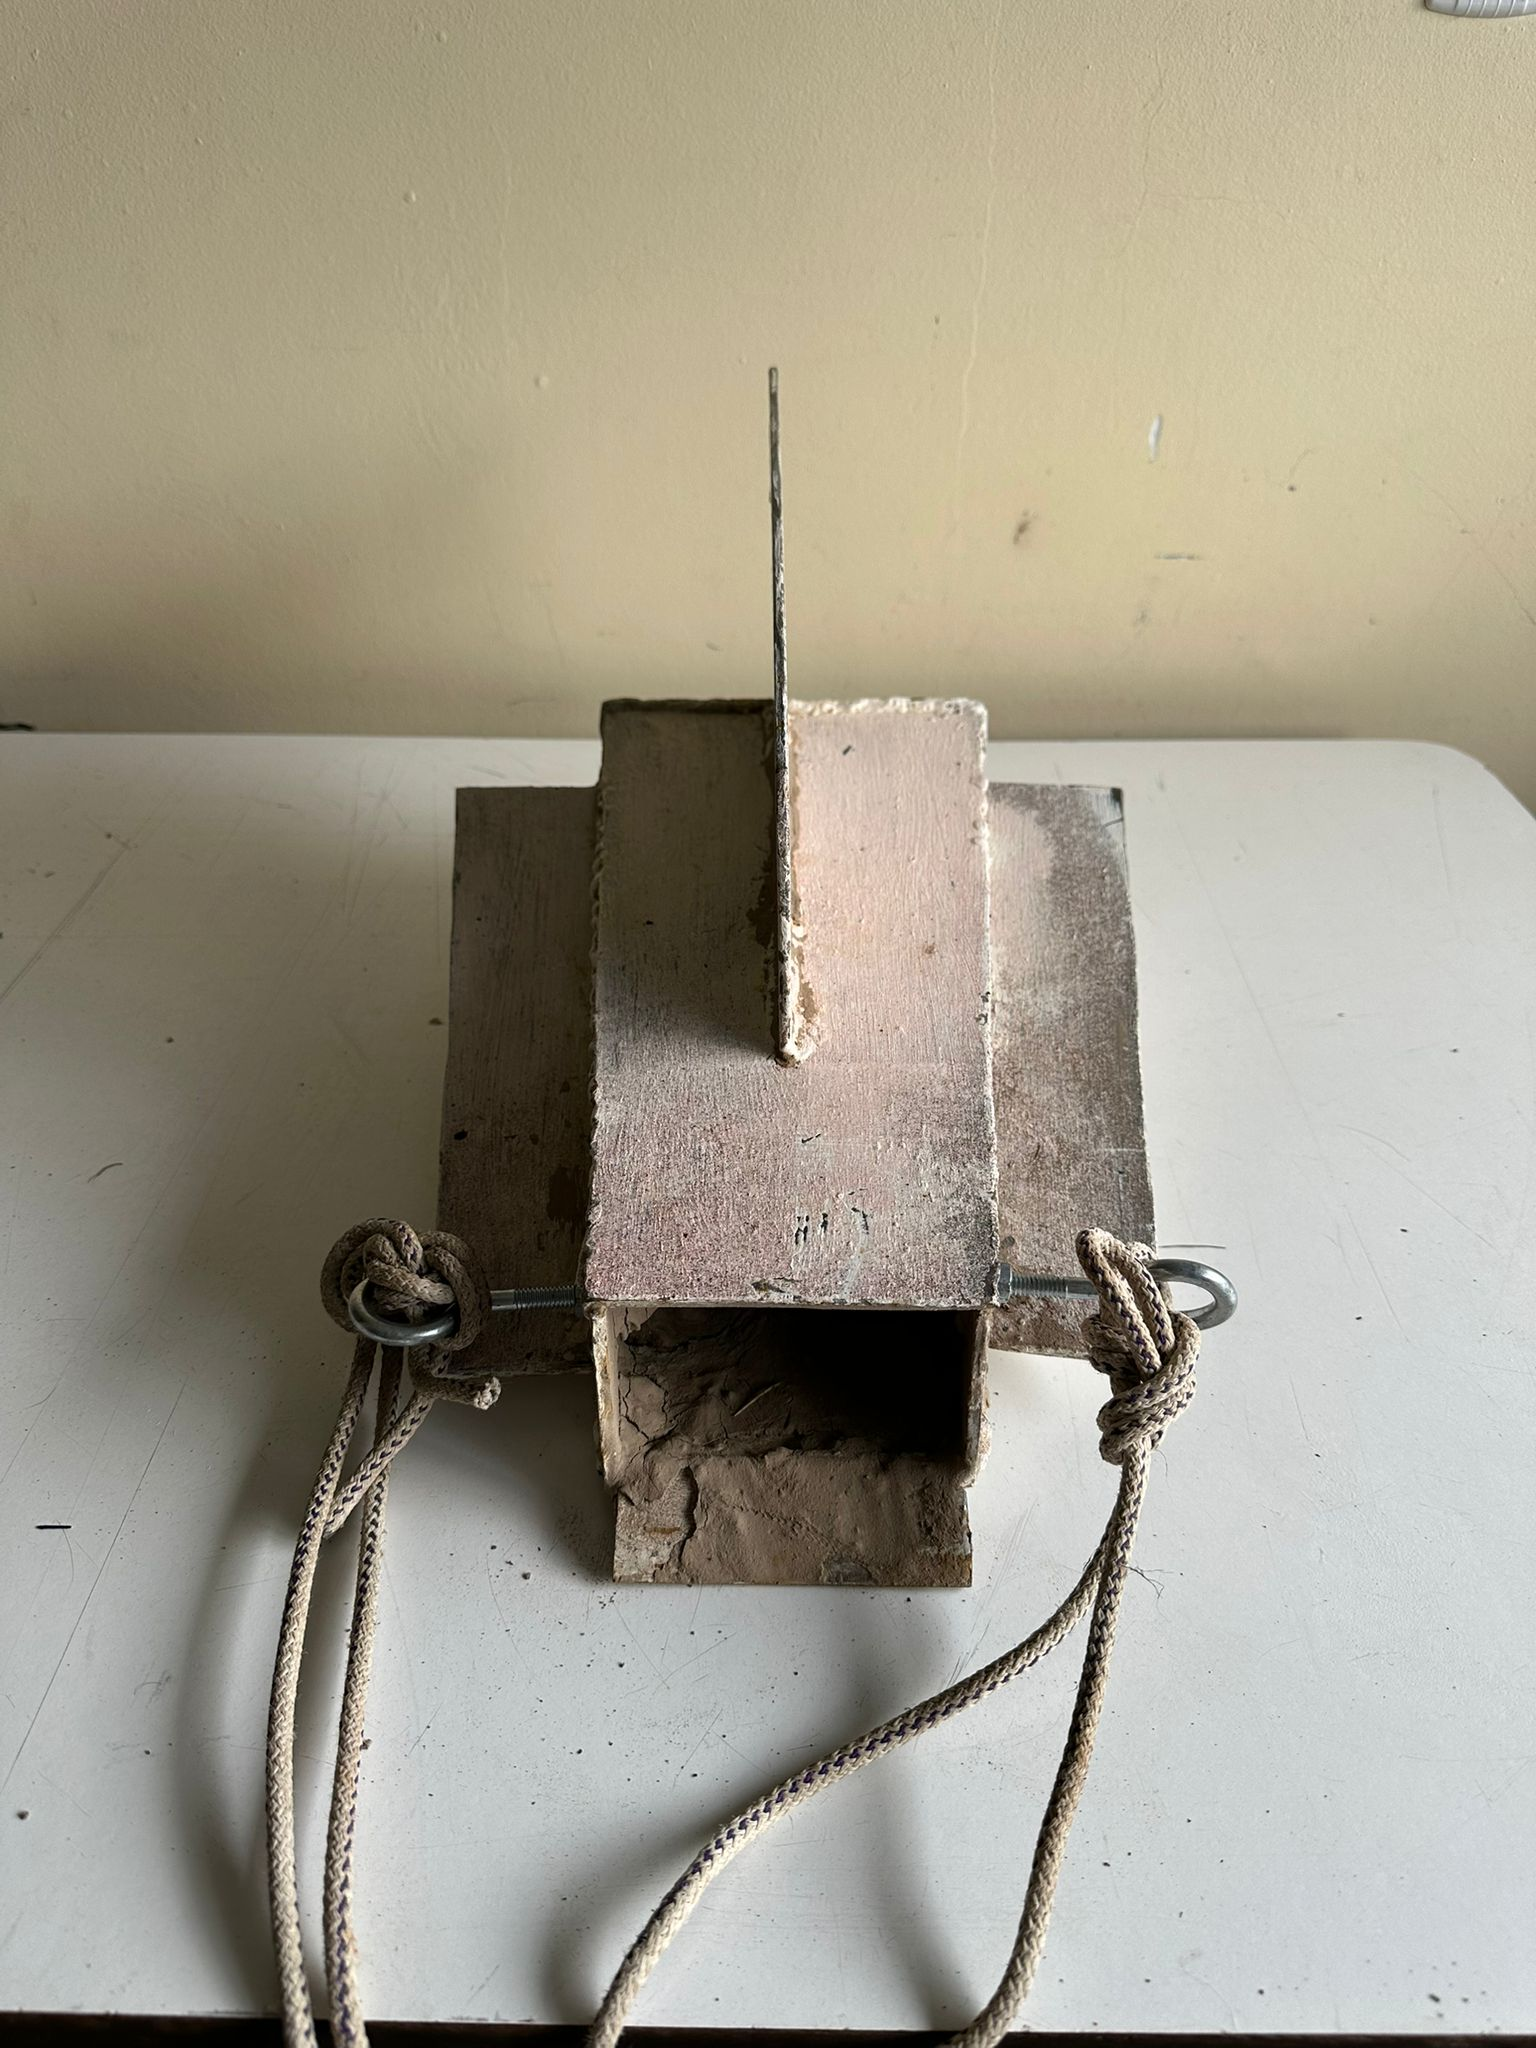
\includegraphics[width=\linewidth]{figures/appendixE/metalcontainer.jpg}
        \caption{Metal Container used}
    \end{subfigure}\hfill
    \begin{subfigure}{0.48\textwidth}
        \centering
        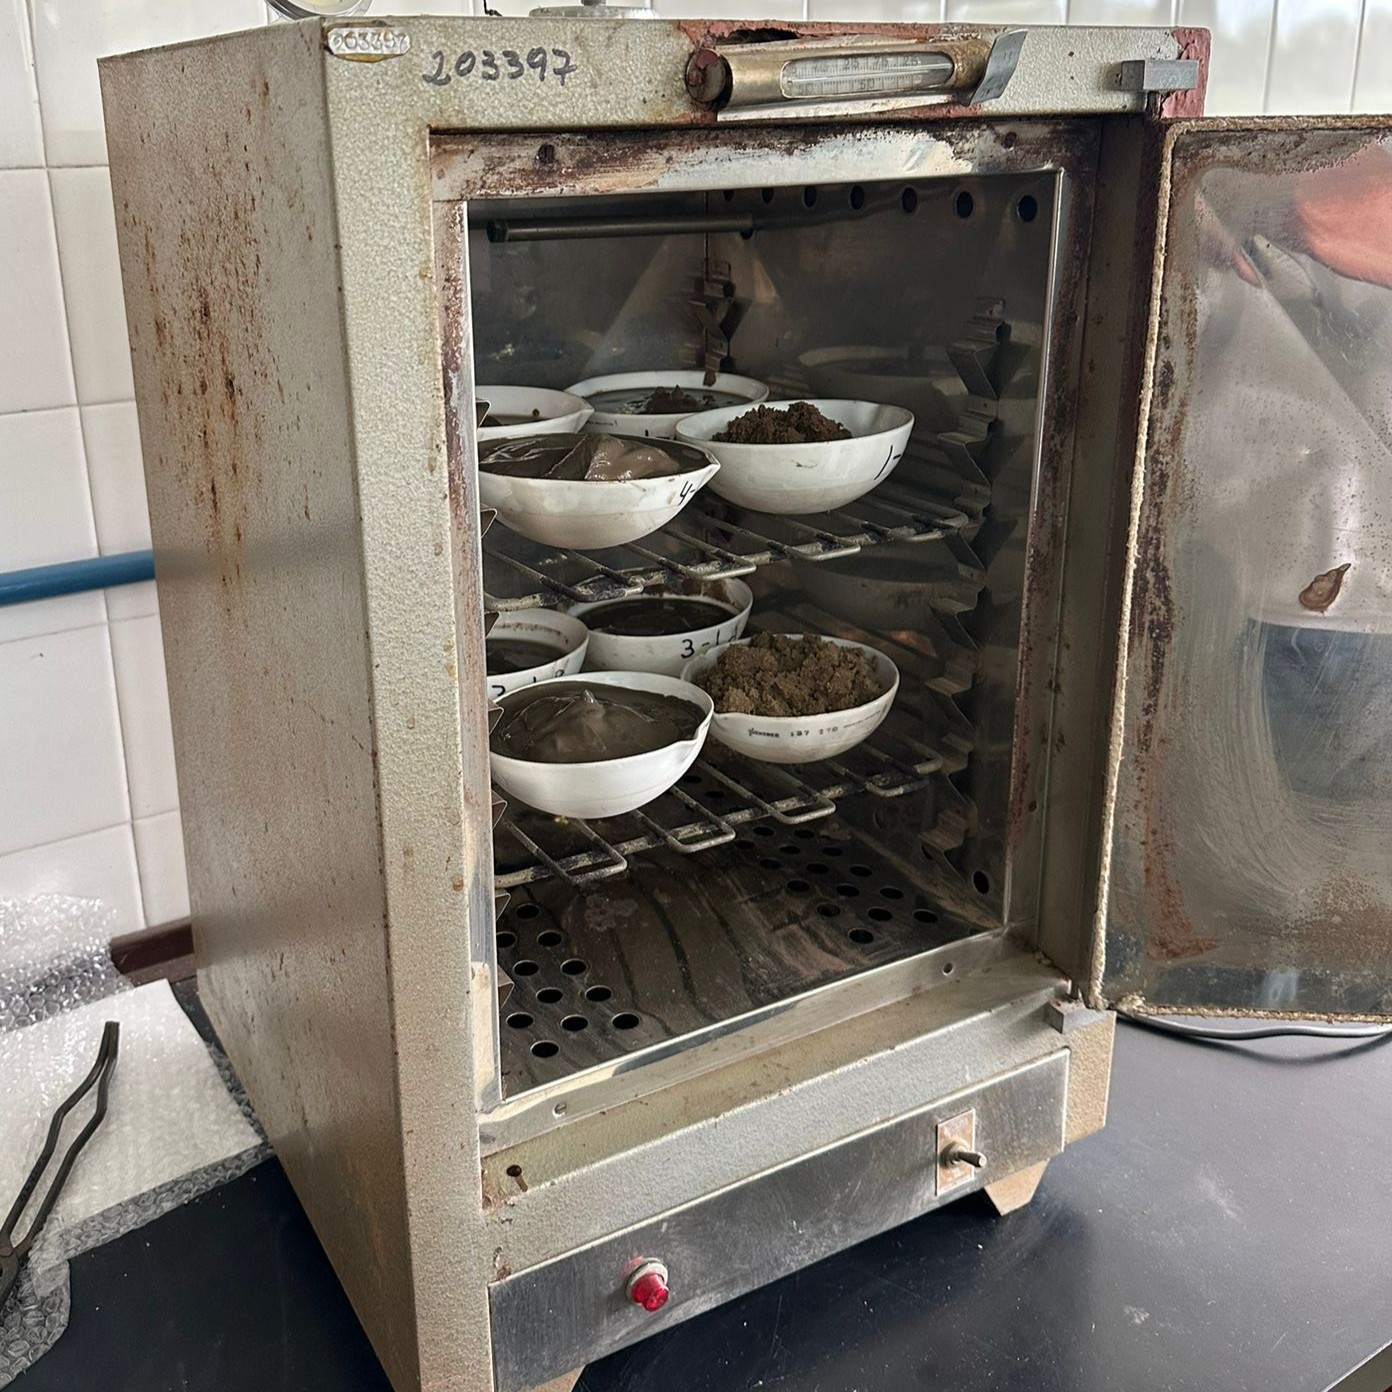
\includegraphics[width=\linewidth]{figures/appendixE/oven.jpg}
        \caption{Oven to dry samples}
    \end{subfigure}

    \caption{Bed Load Measurements}
    \label{fig:bed-load}
\end{figure}


The bed load samples were all weighed before they were put in the oven. There are 7 samples collected at 4 different locations. The first three locations are the cross sections around the extracting point in the bifurcation of the Paraná Guazú with the Talabera river. For these three cross sections two samples were taken from the soil, one at 10 meters depth and one at 15 meters depth, approximately. 
The last sample was taken at 10 meters depth in the cross section upstream close to Puerto Ibicuy. 

All samples were sieved with six different sizes of sieves. The sieving was done 10 minutes per sample. Before the sieving, the samples also been crushed to get the particles loose from clustering. The sieving machine is presented in Figure \ref{fig:siev} The whole collection of the annotated samples can be seen in Appendix \ref{appendix:Lab data}.

\begin{figure}[H]
    \centering
    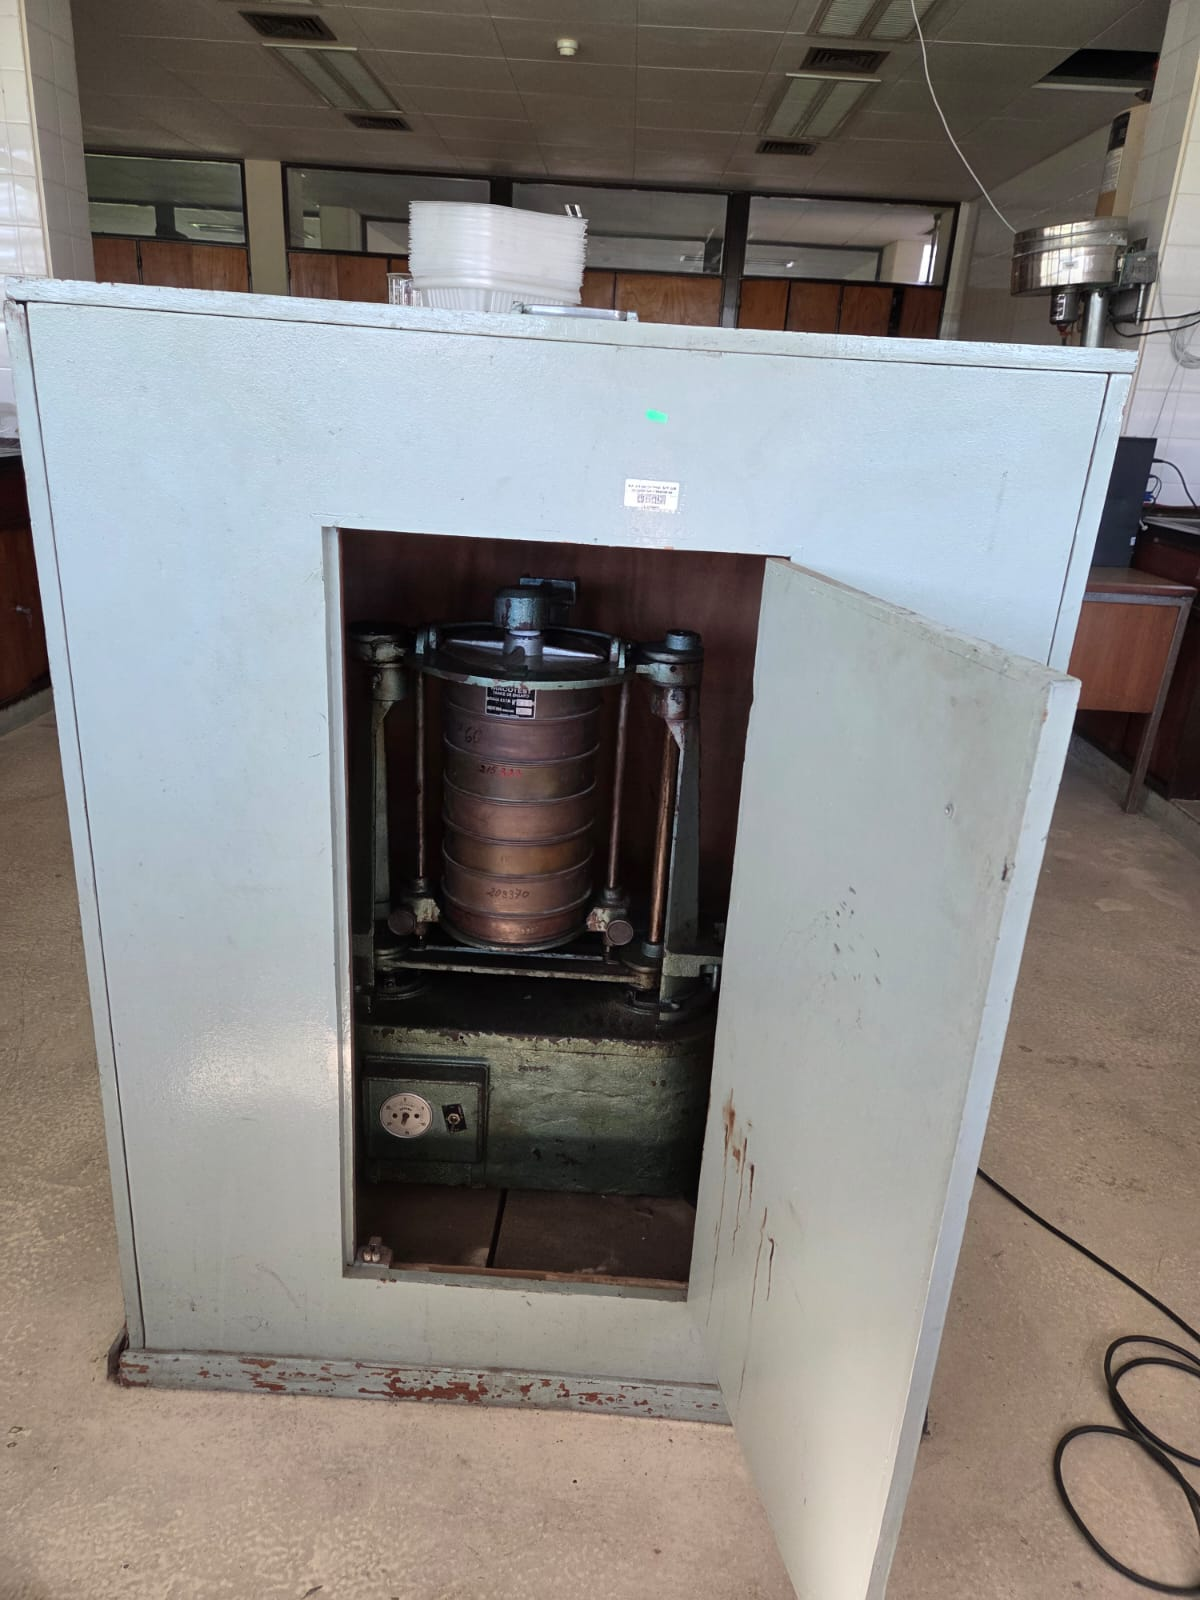
\includegraphics[width=0.5\linewidth]{figures//ch3/siev.png}
    \caption{Sieving machine}
    \label{fig:siev}
\end{figure}


\subsection{Locations of interest}
The locations are divided in two different interest. The measurements locations and the bank erosion locations. Firstly are the measurements locations prescribed and secondly are the bank erosion locations prescribed. 

The measurement campaign was divided into two main locations. The first location, contains a number of cross sections and sediment samples recorded at the confluence of the Talabera and the Paraná Guazú. Figure \ref{fig:measurements day1} shows a summary of the performed measurements. In total, three sections were studied with the following measurements per cross section:
\begin{itemize}
    \item 2 ADCP profiles, yielding bathymetry, discharge and flow velocity
    \item 2 bed load samples at different locations with different depths
    \item 5 suspended sediment samples at a single location with varying depths
\end{itemize}

\begin{figure}[H]
    \centering
    \includegraphics[width=0.75\linewidth]{figures/ch4/day1.png}
    \caption{Measurement locations Day 1}
    \label{fig:measurements day1}
\end{figure}

The second location, contains measurements at Puerto Ibicuy. There, some cross sections were measured in the vicinity of the confluence of the Ibicuy and the Paraná Guazú. In addition, the echosounder was active all day long. Its recorded tracks can be found in Figure \ref{fig:measurements day2}. The following results have been found on day 2:
\begin{itemize}
    \item 6 ADCP profiles. 2 profiles each for the most upstream and most downstream cross section, respectively. 1 profile for those in between. 
    \item 1 bed load sample near Puerto Ibicuy
    \item 2 longitudinal profiles along the confluence of Talabera and Paraná Guazú, measured at the beginning and end of the day to study dune migration
\end{itemize}

\begin{figure}[H]
    \centering
    \includegraphics[width=0.75\linewidth]{figures/ch4/day2.png}
    \caption{Measurement locations Day 2}
    \label{fig:measurements day2}
\end{figure}

In this paragraph, the methodology is explained as to how one has studied this matter, and how the data was found to get to conclusions.

During the field work it was noticed through the interviews that a significant amount of people living along the riverside were affected by bank erosion \ref{chap:interviews}. The research group took multiple pictures from the actual conditions in 2025, so that a comparison could be established once older data was obtained. From what was seen, the land was highly eroded, some trees were on the verge of being in the water, while others were already sucked up by the river. This can be seen in the Figures \ref{bankerosion} below taken during the field trip.

\begin{figure}[H]
    \centering
    \begin{subfigure}[b]{0.6\textwidth}
        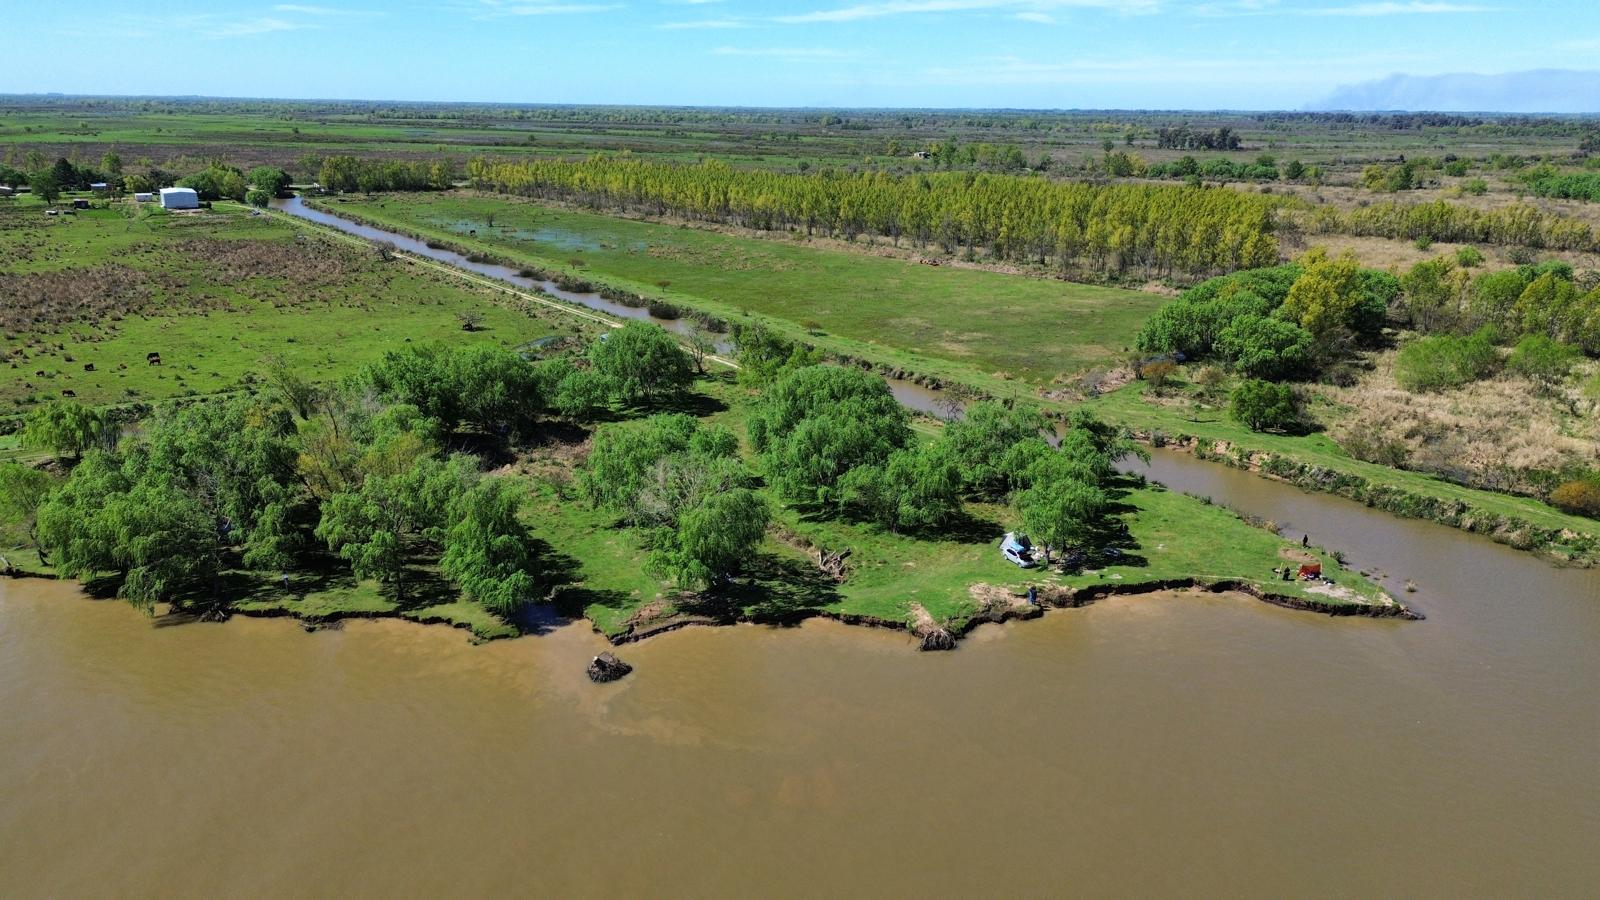
\includegraphics[width=\linewidth, height=6cm]{figures/ch4/bankerosioncamping.jpg}
        \caption{Bank Erosion La Blanqueada}
        
    \end{subfigure}
    
    \vspace{0.5cm}
    

    \begin{subfigure}[b]{0.6\textwidth}
        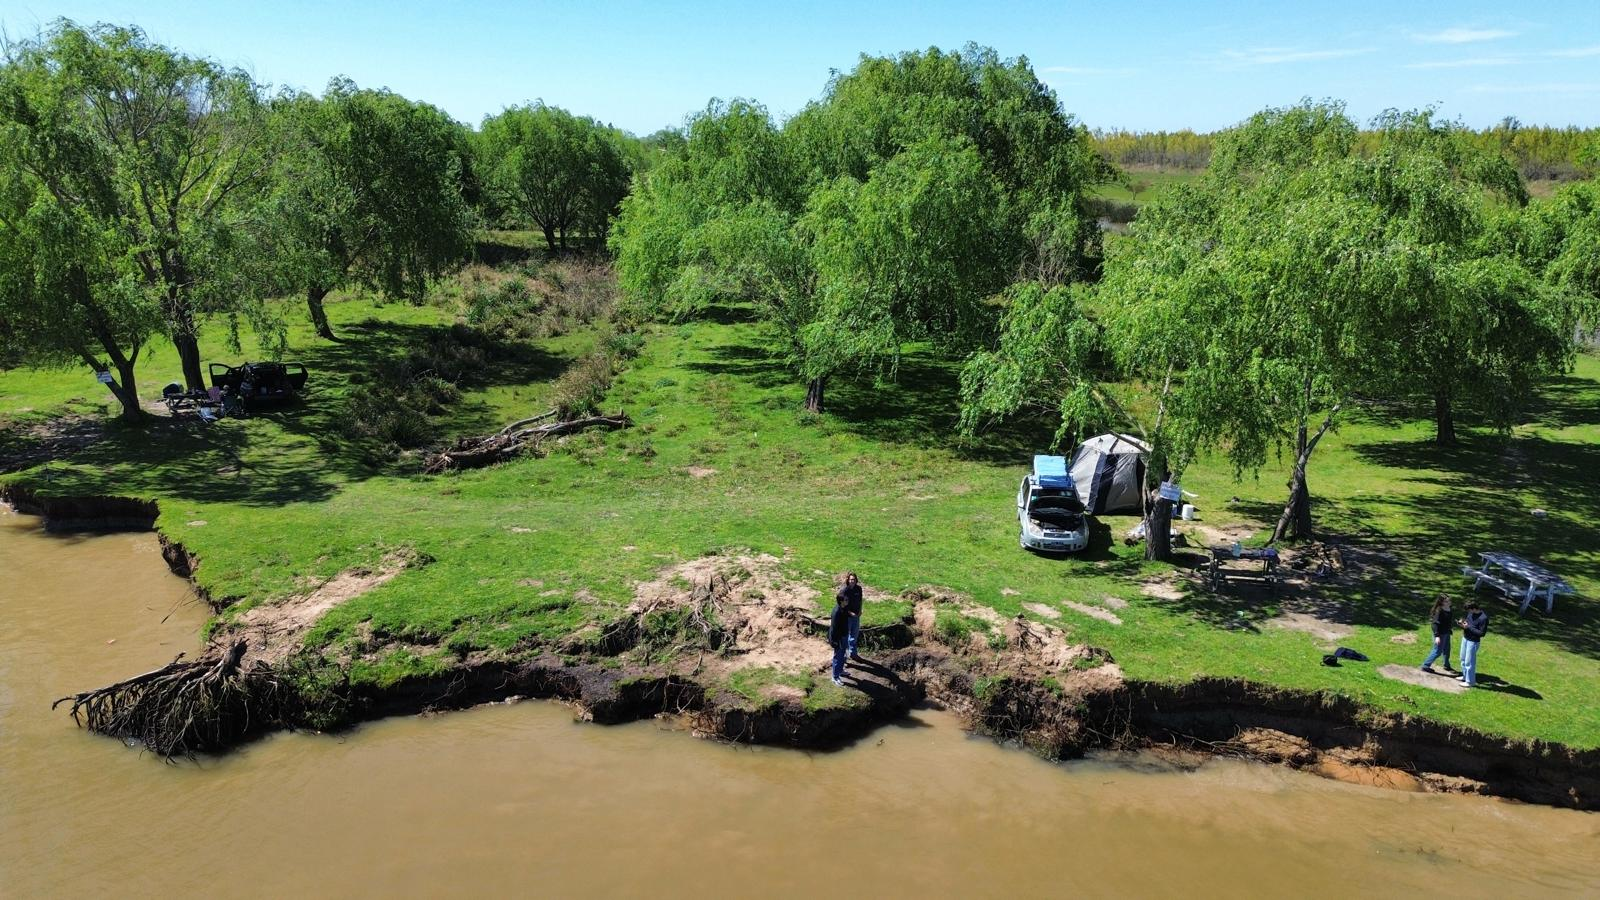
\includegraphics[width=\linewidth, height=6cm]{figures/ch4/bankerosioncamping2.jpg}
        \caption{Bank Erosion Closeup}
        
    \end{subfigure}
    \caption{Bank Erosion Shots from Field Work}
    \label{fig:Bank Erosion shots from field work}
\end{figure}
\label{bankerosion}


From the owner of the Camping la Blanqueada and the landowner a few hundred meters from the same location, it was informed that they saw their land was erode up to 30 meters every few years. This was quite a serious take and therefore it questioned us leading to an initiative to study this narrative.

From the Aqua Monitor Software, one can establish which regions are of interest in a broad scope surrounding the Paraná Guazú bend near Puerto Constanza. Decreasing the scope makes it relevant to investigate the actual areas and lengths of land that have been subject to these water gains. Therefore, it was chosen to investigate further into the details of the coast erosion with Google Earth. The satellite database of Deltares was used for different time stamps, starting from 1984. The reason behind this is that the Deltares Aqua Monitor is a tool using Google Earth Engine, containing satellite imagery from 1984 until today. The choice was made to analyze the data in time batches of 10 years from 1985 until 2005, then in 5 years from 2005 to 2015, and lastly every 2.5 years in the last decade.

A preview of the maps can be seen in Figure \ref{Aqua Monitor Water Changes 1985-2025}below, but the final analysis and conclusions are explained in Chapter \ref{chap:hydroanalysis}. 

\begin{figure}[H]
    \centering
    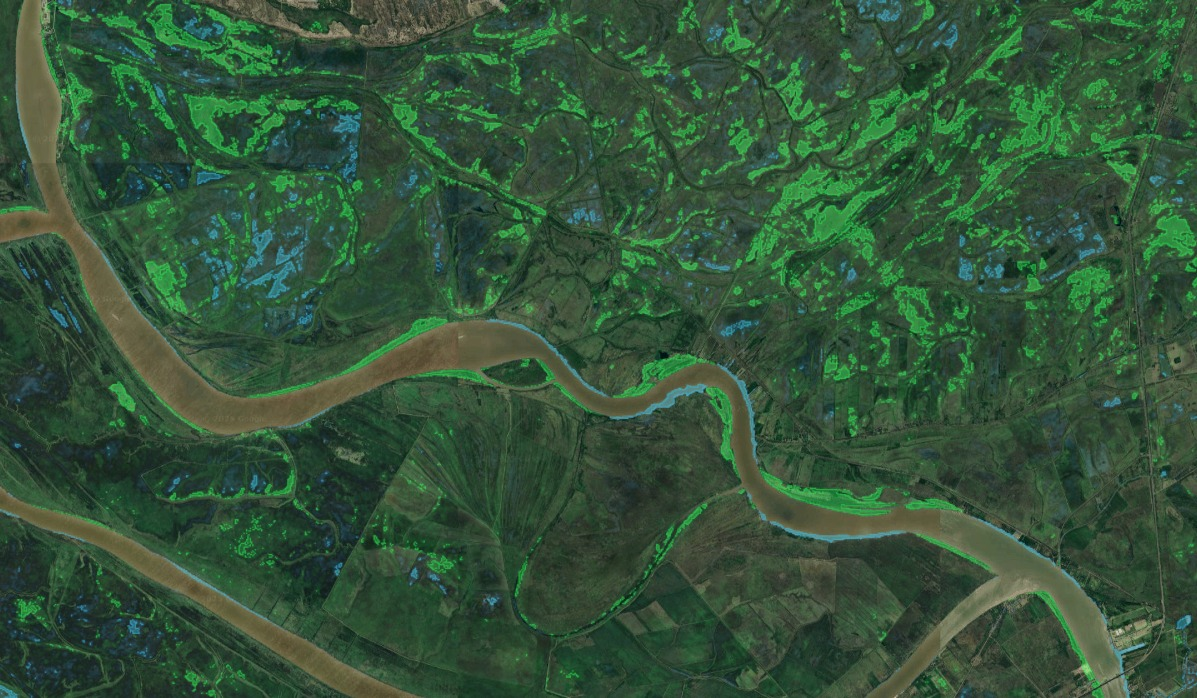
\includegraphics[width=0.75\linewidth]{figures/ch4/1985-2025.jpg}
    \caption{Aqua Monitor Water Changes 1985-2025}
\end{figure}
\label{Aqua Monitor Water Changes 1985-2025}

For more clarity, the green parts of Figure \ref{Aqua Monitor Water Changes 1985-2025} are water losses and the blue parts are water gains over time. For the whole collection of Figures see Appendix \ref{Appendix: Satellite Data}.

\section{Modelling approach}
This section explains the approach that was used to make the Delft 3D model and the sheet pile model. These models are made to answer the research question. 

Firstly, ..... .Using the flow velocity one can derive the concentration of the sediment in the study area. This can be done for several locations in order to get an idea of the quantities of sediment that come in through the Rio Ibicuy. Then the last critical point will help us determine the continuation of the concentration of the sediment in the Rio Parana so that any inconsistencies can be linked with the amount of extracted sand in the intersection of the Parana Guazu and Rio Talabera (in the middle of the three critical points on the right hand side of Figure 4.2).

A mathematical expression/derivation will be explained.....

Secondly, there is made a sheet pile model. For the design of the sheet pile model as a mitigation strategy for bank erosion, a flow chart is used as a methodology. The flow chart shown in Figure \ref{fig:flow_chart} is divided into three phases. In the first phase, data analysis, research will be performed to gain a better understanding of the critical locations and parameters necessary for the design. Apart from these, structural regulations, stated in the Eurocode, were specified. 

\textit{Data analysis}

\begin{itemize}
    \item Aqua Monitor will be used to alert critical erosion points along the Paraná Guazú, while during the field trip, these critical points will be visited to better understand the situation.
    \item Literature research were performed to assess critical parameters and data for the sheet pile model.
    \begin{itemize}
        \item Soil conditions include borehole findings to assess the different layers and the accompanying soil parameters.
        \item Hydraulic parameters include bathymetry findings provided by INA to assess water level and river bed formation along the banks.
        \item Structural standards and regulations, the Eurocode, is used to perform structural verifications regarding the ultimate and serviceability limit state.
    \end{itemize}
\end{itemize}   

In the second phase of the sheet pile model, a sheet pile type were chosen and the gathered data is used to analyse the earth and hydrostatic pressure. The method chosen is the simplified Padfield and Mair method, which provides a plan to design a sheet pile. Combining the method and analysis, the sheet pile model and its unknown design parameters, including structural verifications, can be drawn. 

\textit{Design analysis}

\begin{itemize}
    \item Multiple design methods were reviewed and the simplified Padfield and Mair will be applied to perform the earth and hydraulic pressure analysis.
    \item The procedure for calculating the embedding depth of the sheet pile is related to the method of the simplified Padfield and Mair, and the pressure diagrams for the earth and hydrostatic pressure is provided by Python Code.
    \item The sheet pile design, made in Python Code, is a combination of both earth and hydrostatic pressure.
    \item Structural verifications of shear force, bending moment, and deflection is compared with the resistance of the chosen sheet pile profile.
\end{itemize}

The final phase will conduct the sustainability aspects for the sheet pile model. The final phase will be explained in more detail in the following.

\textit{Sustainability analysis}

\begin{itemize}
    \item The sustainability of the sheet pile profile is assessed and a suitable profile is selected. 
\end{itemize}

\begin{figure}[H]
    \centering
    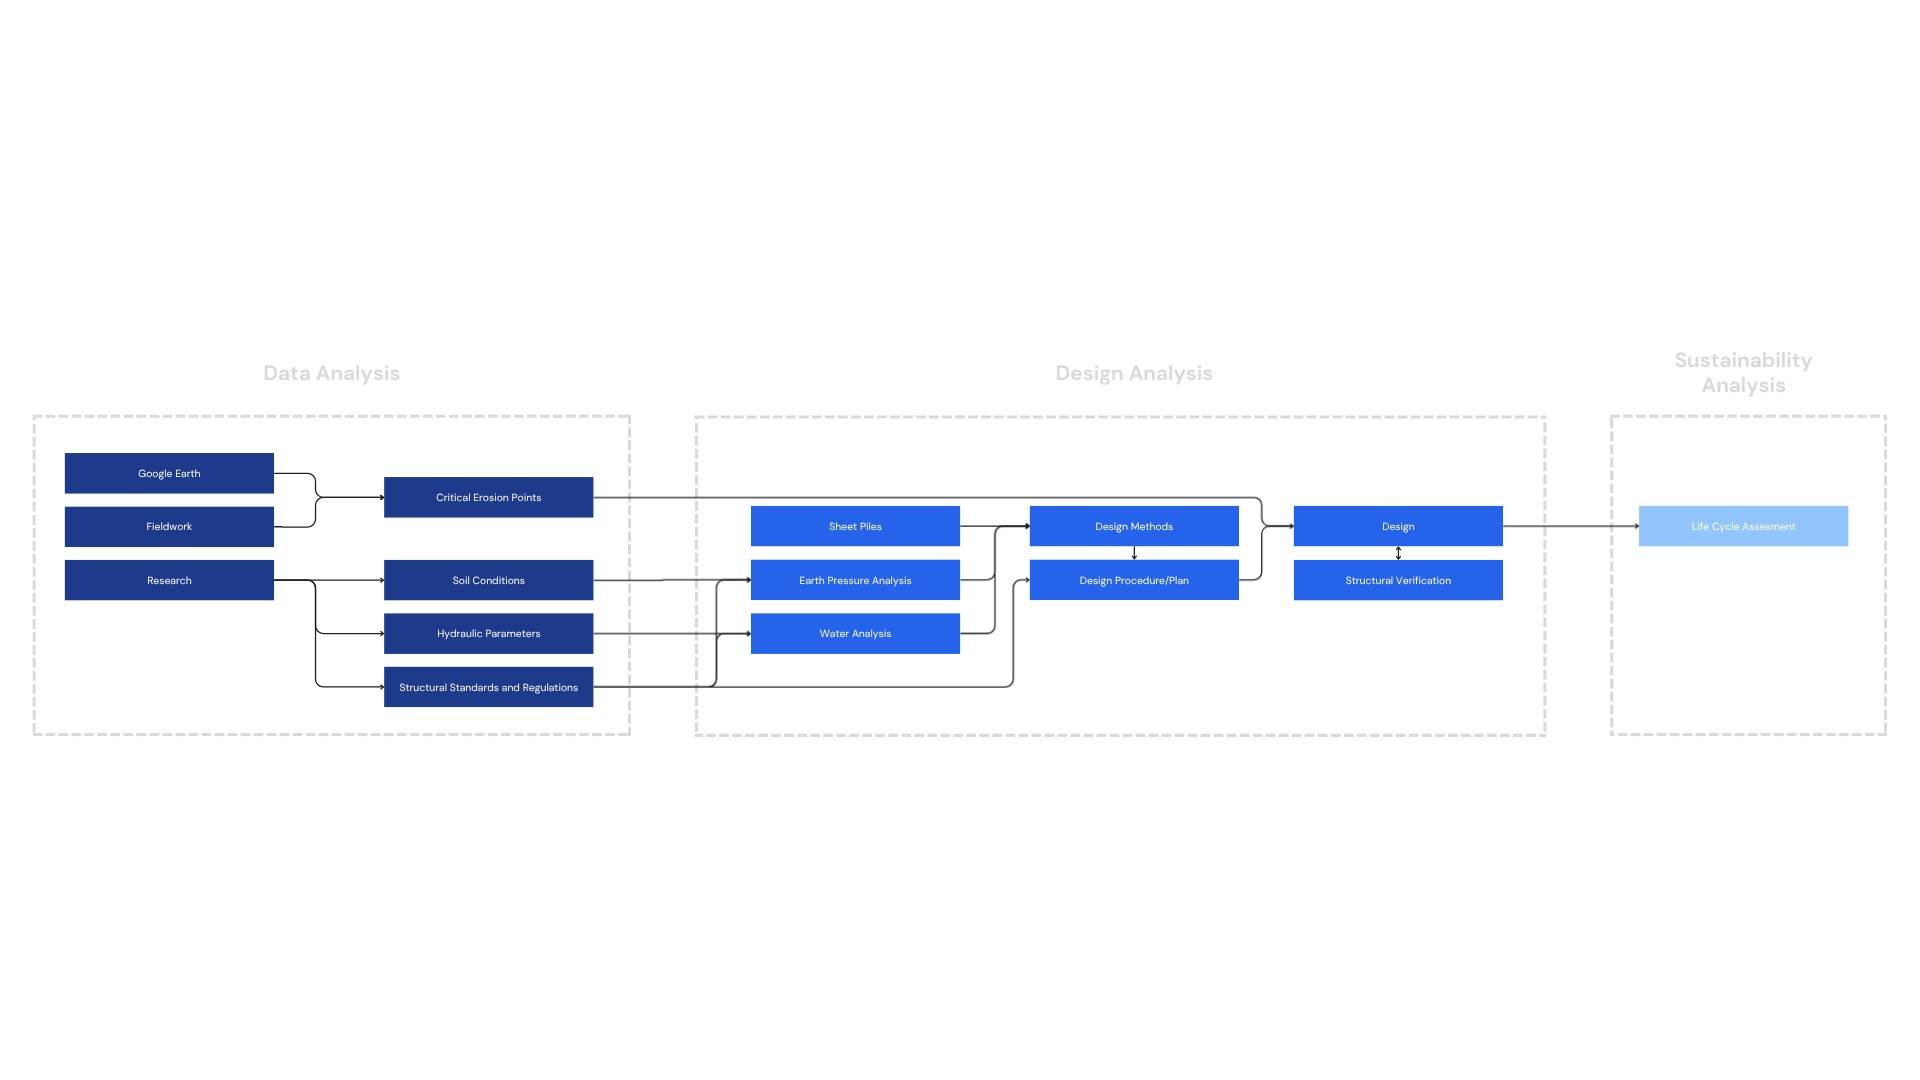
\includegraphics[width=\linewidth]{figures/ch3/FlowChart Structural (2).png}
    \caption{Flow chart sheet pile model}
    \label{fig:flow_chart}
\end{figure}



